%\documentclass[11pt,a4paper,oneside,twocolumn,titlepage]{ieeeconf} 
\documentclass[11pt,a4paper,oneside,twocolumn]{ieeeconf} 
\usepackage[T1]{fontenc}

%%%%%%%%%%%%%%%%%%%%%%%%%%%%
\usepackage[utf8]{inputenc}
\usepackage[english]{babel}
\usepackage[english]{varioref}
\usepackage{microtype}
\usepackage{titling}
\usepackage[autostyle,italian=guillemets]{csquotes} %stabilire stile quote

\usepackage[backend=biber,bibstyle=numeric,citestyle=numeric-comp]{biblatex}
\addbibresource{bibliography.bib}

\usepackage{quoting}
\quotingsetup{font=small, font=itshape}

\usepackage{booktabs}
\usepackage{tabularx}
\usepackage{caption}
\captionsetup{tableposition=top,figureposition=bottom,font=small,format=hang,labelfont={sf,bf}}
\newcolumntype{Y}{>{\centering\arraybackslash}X}
\usepackage{multirow}
\usepackage{subfig}

\usepackage{fancyhdr}

\usepackage{amsmath}
\usepackage{amssymb}
\usepackage{mathtools}
\usepackage{centernot}
\usepackage{braket}
\usepackage{amsthm}

\usepackage[output-decimal-marker={.}]{siunitx}

\newcommand{\omissis}{[\textellipsis\unkern]}
\usepackage{eurosym}

\usepackage{varwidth}
\newcolumntype{M}{>{\begin{varwidth}{3cm}}c<{\end{varwidth}}} %M is for Maximal column
\providecommand{\keywords}[1]
{
	\small  
	\textbf{\textit{Keywords---}} #1
}

%Overleaf porting
\usepackage{tikz}
\usepackage{enumitem}

\usepackage{definitions}

\usepackage{hyperref}
\hypersetup{
	pdfpagemode={UseOutlines},
	bookmarksopen,
	pdfstartview={FitH},
	colorlinks,
	linkcolor={blue},
	citecolor={blue},
	urlcolor={blue}
}

\begin{document}
	\author{
		Andrea Terlizzi\thanks{Andrea Terlizzi, Computer Science Department, Università degli Studi di Salerno},		
		Mattia Limone\thanks{Mattia Limone, Computer Science Department, Università degli Studi di Salerno}, 
		Carmine Iannotti\thanks{Carmine Iannotti, Computer Science Department, Università degli Studi di Salerno} ,  	
		Luca Strefezza\thanks{Luca Strefezza, Computer Science Department, Università degli Studi di Salerno}
		}	
	\thanksmarkseries{arabic}
	\title{A Deep LSTM-CNN-HMM Neural Network\\system for Speaker Identification}
	%\date{}
	\maketitle
	
	%{
		%\hypersetup{linkcolor=black}
		%\tableofcontents
	%}
	
	\begin{abstract}
	Deep learning approaches are progressively gaining popularity as alternative to HMM models for speaker identification. Promising results have been obtained with Convolutional Neural Networks (CNNs) fed by raw speech samples or raw spectral features, although this methodology does not fully take into account the temporal sequence in which speech is produced.
	
	DNN-HMM (Deep Neural Network-Hidden Markov Model) is a methodology that combines the statistical modeling power of HMMs with the learning power of deep neural networks. While this technique has seen wide use in speech recognition field, few studies tried to apply it to speaker identification tasks.
	
	This study proposes a novel approach to the DNN-HMM methodology for text-independent speaker identification, involving the use of both convolutional and Long-Short-Term-Memory (LSTM) networks, in order to extract both high-level features from the entire audio and temporal-wise features from each frame, which are then used to predict the emission probabilities of an HMM.
	
	The experiments conducted on the TIMIT dataset showed very promising results, suggesting that the proposed non-sequential architecture may converge faster and perform better than other known methods, if properly tuned.
\end{abstract}
	\section{Introduction}
Speaker identification (SI) tasks can be classified in two big groups: text-dependent and text-independent.

In the first type of task, identification is done with the help of a passphrase that the individual has to pronounce so that the system can recognize him or her, based both on the audio features extracted by the speaker audio utterances and the spoken words.

Text-independent SI, on the other hand, is entirely based on features extracted from audios, and cannot rely on either the phonetic structure of the spoken sentence or its content.

This study, inspired by recent and multiple encouraging results in the application of deep neural networks to text-independent SI \cite{si:lstm}, sometimes used in conjunction with other types of models such as Hidden Markov Models (HMMs) or Gaussian Mixture Models (GMMs) (in so-called "hybrid approaches" \cite{si:dnnhmm}), proposes a new approach to DNN-HMM methodology applied to this task, involving the use of both deep Long-Short-Term-Memory networks (LSTMs) and Convolutional Neural Networks (CNNs).

To our knowledge, DNN-HMM hybrid approaches are still largely untested in text-independent SI, which is one of the reasons why we decided to use LSTM Neural Networks and CNNs, both of which fit perfectly the SI task, as widely demonstrated in the literature \cite{si:cnn} \cite{si:lstm}.

The study, conducted on the TIMIT dataset, takes advantage of some of the most historically appreciated and used features in the audio and speech processing literature, such as MFCCs, LPCCs, and log-scaled Mel spectrum.

The work is organized as follows: section \vref{sec:dataset} describes the used dataset in detail, presenting the file structure and its composition; sections \vref{sec:preprocessing}, \vref{sec:feature_extraction}, \vref{sec:acoustic_modeling} explain the preprocessing, feature extraction and HMM acoustic modeling steps made prior to the model training; sections \vref{sec:dnnhmm} and \vref{sec:architecture} describe the applied DNN-HMM technique and the proposed neural network architecture; finally, sections \vref{sec:pre_training} and \vref{sec:results} describe the experiment carried out in detail, starting with the pre-training phase of the model layers, going through the training of the model and finally arriving at the results obtained and possible future developments. 
	\section{Dataset}\label{sec:dataset}

In this research we worked on the \textit{DARPA TIMIT - Acoustic-Phonetic Continuous Speech Corpus}~\cite{garofolo:timit}. This dataset has been designed to provide speech data for the acquisition of acoustic-phonetic knowledge and for the development and evaluation of automatic speech recognition (ASR) systems. TIMIT has resulted from the joint efforts of several sites under sponsorship of the Defense Advanced Research Projects Agency - Information Science and Technology Office (DARPA-ISTO). Text corpus design was a joint exertion among the Massachusetts Institute of Technology (MIT), Stanford Research Institute (SRI), and Texas Instruments (TI).

\subsection{Speaker Distribution}
TIMIT contains a total of 6300 sentences, 10 sentences for each of 630 speakers from 8 major dialect regions of the United States. Table \vref{tab:dialect_distribution} shows the number of speakers for the 8 dialect regions, broken down by sex. A speaker's dialect region is the geographical area of the U.S. in which they lived during their childhood years. The geographical areas correspond with recognized dialect regions in U.S., with the exception of the Western region (DR7) in which dialect boundaries are not known with any confidence, and dialect region 8 (DR8), where the speakers moved around a lot during their childhood.

\begin{table}
	\caption{Dialect distribution of speakers.}
	\label{tab:dialect_distribution}
	\centering
	\begin{tabularx}{0.5\textwidth}{llll}
		\toprule
		\textbf{DR} & \textbf{Male} & \textbf{Female} & \textbf{Total} \\
		\midrule
		1 & 31 (63\%) & 18 (27\%) & 49 (8\%) \\
		2 & 71 (70\%) & 31 (30\%) & 102 (16\%) \\
		3 & 79 (67\%) & 23 (23\%) & 102 (16\%) \\
		4 & 69 (69\%) & 31 (31\%) & 100 (16\%) \\
		5 & 62 (63\%) & 36 (37\%) & 98 (16\%) \\
		6 & 30 (65\%) & 16 (35\%) & 46 (7\%) \\
		7 & 74 (74\%) & 26 (26\%) & 100 (16\%) \\
		8 & 22 (67\%) & 11 (33\%) & 33 (5\%) \\
		\midrule
		All & 438 (70\%) & 192 (30\%) & 630 (100\%) \\
		\bottomrule
	\end{tabularx}
\end{table}

\subsection{File Structure}
The speech and associated data is organized in the dataset according to the following directory hierarchy:
\begin{verbatim}
	/data/
		<USAGE>/
			<DIALECT>/
				<SEX><SPEAKER_ID>/
					<SENTENCE_ID>.<FILE_TYPE>
\end{verbatim}
where:
\begin{itemize}
	\item \verb!usage = train | test!;
	\item \verb|dialect = DRi|, \verb*|i| $\in \{1, ..., 8\}$;
	\item \verb!sex = M | F!;
	\item \verb|speaker_id = <initials><digit>|:
	\begin{itemize}
		\item \verb|initials|: speaker initials, 3 capital letters;
		\item \verb|digit|: number between $0$ and $9$ to differentiate speakers with identical initials;
	\end{itemize}
	\item \verb|sentence_id =| \\ \verb|= <text_type><sentence_number>|:
	\begin{itemize}
		\item \verb!text_type = SA | SI | SX!;
		\item \verb|sentence_number|: $1 ... 2342$;
	\end{itemize}
	\item \verb!file_type:! \\ \quad \verb!wav | txt | wrd | phn!
\end{itemize}
The three values that \verb|text_type| can assume stands for dialect sentences (SA), phonetically-compact sentences (SX) and phonetically-diverse sentences (SI). Even though important in speech recognition, these data were not particularly relevant during execution of the experiments conducted in this study, which is focused on text-independent SI task.

Finally, all the files of type .txt, .wrd and .phn are transcription files, not used in the context of our work.

The following is an example of the structure described above: \verb*|/data/train/DR1/FCJF0/SA1.wav|, indicating: training set, dialect region 1, female speaker with ID CJF0, sentence text "SA1", speech waveform file.

\subsection{Suggested Training/Test Subdivision}
TIMIT comes with texts and speakers already subdivided into suggested training and test sets. This subdivision has evolved over time to meet different criteria (as described by the authors~\cite[20]{garofolo:timit}). In the context of this research, the proposed subdivision has been ignored in order to create a new one more suitable for its intended purposes, as described in section \vref{sec:train_test_subdivision}.
	\section{Preprocessing}\label{sec:preprocessing}
Preprocessing is a critical step in any project related to machine learning, even more so in systems where background-noise or silence in training/testing audio signals is completely undesirable~\cite{jahangir:review}. SI task requires efficient feature extraction approaches from speech signals, because most of the spoken portion includes speaker-related attributes useful to the identification.

TIMIT being a dataset recorded in a controlled environment, doesn't need overly complicated preprocessing operations before moving on to those typical of audio signals processing and that intersect the feature extraction phase, such as framing, windowing, spectrogram computation etc. For this reason, we just applied a limited silence removal, described below, while the operations that intersect the feature extraction phase are described in the appropriate section (\vref{sec:feature_extraction}).

\subsection{Silence Removal}
Silence removal is used to eliminate the unvoiced and silent portion of the speech signal. 
For this purpose, input signal is divided into small segments (frames) and root mean square 
(RMS) of each individual segment is calculated and compared with a specific threshold value~\cite{asadullah:silence_removal}.

RMS value of each individual segment can be calculated as:
$$
\RMS_{\Segment}=\sqrt{\mean(\Segment)^{2}} \text{, }
$$
while threshold value is computed as:
$$
R_{t h}=\frac{\mu+v}{2} \text{, }
$$
where $v$ is the minimum RMS value of $K$ voiced signals and $\mu$ is the mean RMS value of $K$ unvoiced signals. The formula to compute $\mu$ is the following:
$$
\mu=\frac{1}{K} \sum_{i=1}^{K} \RMS_{\text{Unvoiced}}
$$
If $\RMS_{\Segment}$ of individual segment is less than $R_{th}$ then the segment id deleted. Similarly all the segments are compared with threshold value and system will delete all the unvoiced portion from the input speech signal. That being said, the silence removal function is expressed as:
$$
f(x)=\left\{\begin{array}{c}
	\RMS_{\Segment} > R_{t h}, \text { voiced signal }\\
	\RMS_{\Segment} \leq R_{t h}, \text { silent signal }
\end{array}\right.
$$
As for our study, we only removed silent frames longer than $0.25s$, since shorter silence time slices could represent discriminating characteristics useful in identifying speakers.

\subsection{Dataset Training/Test Subdivision}
\label{sec:train_test_subdivision}

Another fundamental aspect of the preprocessing phase is the dataset split in training and test set.
\\As extensively described in the previous sections, the TIMIT dataset consists of 10 audios per speaker. Since the purpose of the work is speaker identification, it is necessary that audios of each speaker be present in both the training set and the test set, so we opted for the classic 80/20 split, randomly extracting 2 audios for each speaker to be included in the test set, and inserting the remaining 8 in the test set.
	\section{Feature Extraction}
\label{sec:feature_extraction}

Feature extraction is one of the key steps in all supervised learning problems. The resulting feature vector (in numeric form) of the feature extraction step is fed as an input into machine learning algorithms (K-NN, SVM, NB, etc.) for the construction and validation of classification/regression model~\cite{jahangir:review}.

Short-term spectral features are extracted from short frames (\num{20} - \SI{30}{ms}) of speech signals, as the speech signal changes continuously due to the articulation of sounds. As a result of these short frames, the extracted features are perceived to be stationary and preserve the local information. Mel Frequency Cepstral Coefficients (MFCCs) and Linear Predictor Cepstral Coefficients (LPCCs) are the most widely employed short-term spectral features in speaker identification~\cite{jahangir:review}, indeed we could say that cepstral coefficients derived from either linear prediction analysis or a filter bank approach are today still considered the de-facto standard in the audio feature extraction~\cite{rao:spectral}, even if many deep learning-related works \cite{si:sincnet}, \cite{si:lstm}, \cite{si:cnn} have shown how less refined features (raw waveform signals, raw log-spectrograms or Mel-scaled log-spectrum features, ...) can also be just as effective if not better in some cases.

It's important to note that one of the reasons for such success is that spectral features represent phonetic information, since they are derived directly from spectra~\cite{rao:spectral}, and these are the ones that allow a better discerning between speakers. In the next two sections we go in more details about the two aforementioned coefficients and how we used them in our study.

\subsection{MFCCs}
Mel Frequency Cepstral Coefficents (MFCCs) are widely used features in ASR and SI. They were introduced by Davis and Mermelstein in the '80s, and have been state-of-the-art ever since.

As the name suggests, MFCCs are based on the Mel-scale (where \textit{Mel} stands for \textit{melody}), a logarithmic scale devised to map the frequency of a sound on a scale that better reflects the human perception of them. Figure \vref{fig:mel_hz_plot} shows the plot of pitch Mel scale versus Hertz scale, we can note how \SI{1000}{mel} equals \SI{1000}{Hz}.

\begin{figure}
	\includegraphics[width=0.5\textwidth]{images/mel_hz_plot}
	\caption{Plot of pitch mel scale versus Hertz scale, source~\cite{wiki:mel_scale}.}
	\label{fig:mel_hz_plot}
\end{figure}

The MFCC feature extraction technique basically includes windowing the signal, applying the DFT, taking the log of the magnitude, and then warping the frequencies on a Mel scale, followed by applying the inverse DCT. The detailed description of the various steps involved in the MFCC feature extraction is explained below.

\subsubsection{Pre-Emphasis}
Pre-emphasis refers to filtering that emphasizes the higher frequencies. It is used to balance the spectrum of voiced sounds that have a steep drop in the high frequency range. Usually the glottal source has a slope of about -12 dB/octave. However, when acoustic energy is radiated from the lips, this results in a spectrum rise of about +6 dB/octave. Therefore, pre-distortion removes some of the glottal effects from the vocal tract parameters.

The most commonly used pre-emphasis filter is given by the following transfer function:
$$
H(z)=1-b z^{-1}
$$

\subsubsection{Framing}
The speech signal is a slowly time-varying or quasi-stationary signal. For stable acoustic characteristics, speech needs to be examined over a sufficiently short period of time. Therefore, speech analysis must always be carried out on short segments across which the speech signal is assumed to be stationary; usually, it is divided into smaller frames each lasting between 20ms and 40ms.

\subsubsection{Windowing}
Advancing the time window every 10 ms enables the temporal characteristics of individual speech sounds to be tracked, and the 20 ms analysis window is usually sufficient to provide good spectral resolution of these sounds, and at the same time short enough to resolve significant temporal characteristics. The purpose of the overlapping analysis is that each speech sound of the input sequence would be approximately centered at some frame. On each frame, a window is applied to taper the signal towards the frame boundaries. This is done to enhance the harmonics, smooth the edges, and to reduce the edge effect while taking the DFT on the signal.
Hamming window has been used as window shape by considering the next block in feature extraction processing chain and integrates all the closest frequency lines. Let:
\begin{itemize}
    \item $X_n$ = input signal;
    \item $Y_n$ = output signal;
    \item $W_n$ = hamming window;
\end{itemize}
then the resulting windowed signal is:
\begin{center}
$Y_n = X_n \times W_n, \quad n=0,1,2,\ldots,N$
\end{center}

\paragraph{DFT Spectrum}
Each windowed frame is converted into magnitude spectrum by applying DFT.
$$
X(k)=\sum_{n=0}^{N-1} x(n) e^{\frac{-j 2 \pi n k}{N}} ; \quad 0 \leq k \leq N-1
$$

\subsubsection{Mel Spectrum}
Mel spectrum is computed by passing the Fourier-transformed signal through a set of band-pass filters known as Mel-filter bank. A Mel is a unit of measure based on the human ears perceived frequency. It does not correspond linearly to the physical frequency of the tone, as the human auditory system apparently does not perceive pitch linearly~\cite{rao:spectral}. We reported the relationship between Mel-scale and Hertz-scale in figure \vref{fig:mel_hz_plot}. The approximation of Mel from physical frequency can be expressed as:
\begin{equation}\label{eq:1}
	f_{\Mel}=2595 \log _{10}\left(1+\frac{f}{700}\right)
\end{equation}
where $f$ denotes the physical frequency in Hz, and $f_{\Mel}$ denotes the perceived frequency~\cite{deller:dt_processing}.

Filter banks can be implemented in either the time domain or the frequency domain, but in MFCC computation, they are usually implemented in the latter one. The center frequencies of the filters are normally evenly spaced on the frequency axis, however, to mimic the perception of the human ear, a warped axis is implemented, according to the nonlinear function given in eq. \vref{eq:1}. The most commonly used filter shaper is triangular, the triangular filter banks with Mel frequency warping we used is presented in figure \vref{fig:mel_filter_bank}.
\begin{figure}
  \includegraphics[width=0.5\textwidth]{images/mel_filters.png}
  \caption{Mel-filter bank, source~\cite{rao:spectral}}.
  \label{fig:mel_filter_bank}
\end{figure}

The Mel spectrum of the magnitude spectrum $X(k)$ is computed by multiplying the magnitude spectrum by each of the triangular Mel weighting filters:
\begin{equation}\label{eq:2}
s(m)=\sum_{k=0}^{N-1}\left[ \lvert X(k) \rvert ^{2} H_{m}(k)\right] ; \quad 0 \leq m \leq M-1
\end{equation}
where $M$ is the total number of triangular Mel weighting filters. $H_{m}(k)$ is the weight given to the $k$-th energy spectrum bin contributing to the $m$-th output band and is expressed as~\cite{rao:spectral}:
\begin{equation}
	H_{m}(k)=\left\{\begin{array}{cl}
	0, & k<f(m-1) \\ \\
	\frac{2(k-f(m-1))}{f(m)-f(m-1)}, & f(m-1) \leq k \leq f(m) \\ \\
	\frac{2(f(m+1)-k)}{f(m+1)-f(m)}, & f(m)<k \leq f(m+1) \\ \\
	0, & k>f(m+1)
	\end{array}\right.
\end{equation}

\subsubsection{Discrete Cosine Transform}

Since the vocal tract is smooth, the energy levels in adjacent bands tend to be correlated. Before computing the DCT, the Mel spectrum is usually represented on a log scale, then DCT is applied to the transformed mel frequency coefficients to produce a set of cepstral coefficients. This results in a signal in the cepstral domain with a quefrency peak corresponding to the pitch of the signal and a number of formants representing low quefrency peaks~\cite{rao:spectral}.

Since most of the signal information (corresponding to the vocal tract features) is represented by the first few MFCC coefficients, we only selected the first 13, as usual in most literature. As in~\cite{picone:signal_modeling}, extracting only those coefficients ignoring or truncating higher order DCT components is sufficient to obtain a robust system. Finally we report, again from~\cite{picone:signal_modeling}, the final formula for calculating MFCCs involving DCT:
\begin{equation}
	c(n)=\sum_{m=0}^{M-1} \log _{10}(s(m)) \cos \left(\frac{\pi n(m-0.5)}{M}\right)
\end{equation}
with $n=0,1,2, \ldots, C-1$, where $c(n)$ are the cepstral coefficients and $C$ is the number of MFCCs, usually between \num{8} and \num{13}.

\subsubsection{First and Second Order Derivatives}
First and second derivative of each MFCC (also known as delta and delta-delta features) are also taken into account, since they carry additional information about the coefficient variation over time, ending up with 39 coefficients for each frame, which will become the input of our deep learning model.

Delta coefficients tell about the speech rate, while delta-delta coefficients provide information similar to acceleration of speech~\cite{rao:spectral}. The commonly used definition for computing these dynamic parameters (delta features) is:
\begin{equation}
	\Delta c_m(n) = \frac{\sum_{i = -T}^{T} k_i c_m (n + i)}{\sum_{i = -T}^{T}\lvert i \rvert}
\end{equation}
where $c_m(n)$ denotes the $m$-th feature for the $n$-th time frame, $k_i$ is the $i$-th weight and $T$ is the number of successive frames used for computation. Generally $T$ is taken as $2$. The delta-delta coefficients are computed by taking the first order derivative of the delta coefficients~\cite{rao:spectral}.

\subsection{LPCCs}
LPCCs are another type of cepstral coefficients widely used in speech processing~\cite{jahangir:review}. As mentioned in the section~\vref{sec:feature_extraction}, spectral features represent phonetic information, as they are derived directly from spectra. The features extracted from spectra, using the energy values of linearly arranged filter banks, equally emphasize the contribution of all frequency components of a speech signal. In this context, LPCCs are used to capture emotion-specific information manifested through vocal tract features~\cite{rao:spectral}.

As in the case of MFCCs, the Linear Predictive (LP) analysis requires multiple steps, exemplified in the figure \vref{fig:lpc}, that represents the steps from the speech signal to the LPCs (Linear Predictive Coefficients). The next step is to actually extract the cepstral coefficients, as shown in Figure~\vref{fig:lpcc}.
\begin{figure}
	\includegraphics[width=0.5\textwidth]{images/lpc}
	\caption{LPC block diagram.}
	\label{fig:lpc}
\end{figure}
\begin{figure}
	\includegraphics[width=0.5\textwidth]{images/lpcc}
	\caption{LPCC block diagram.}
	\label{fig:lpcc}
\end{figure}

In this work we extracted from the speech signal 13 LPCCs per speech frame of \SI{16}{ms}, using an overlap of \SI{8}{ms} and the \textit{hann} windowing.

\subsubsection{Cepstrum and LPCCs Calculation}

Cepstrum may be obtained using linear prediction analysis of a speech signal. The basic idea behind linear predictive analysis is that the $n$th speech sample can be
estimated by a linear combination of its previous $p$ samples as shown in the following equation~\cite{rao:spectral}:

\begin{multline}
	s(n) \thickapprox a_1s(n - 1) + a_2s(n - 2) +\\+ a_3s(n - 3) + \dots + a_ps(n - p)
\end{multline}
where $a_1, a_2, a_3, \dots$ are assumed to be constants over a speech analysis frame. These are known as predictor coefficients or linear predictive coefficients. These coefficients are used to predict the speech samples, then we can calculate the error as the difference of actual and predicted speech samples, by the following formula:

\begin{equation}
	e(n) = s(n) - \hat{s}(n) = s(n) - \sum_{k = 1}^{p}a_ks(n - k)
\end{equation}
where $e(n)$ is the error in prediction, $s(n)$ is the original speech signal, $\hat{s}(n)$ is a predicted speech signal and $a_k$s are the predictor coefficients.

To compute a unique set of predictor coefficients, the sum of squared differences between the actual and predicted speech samples has to be minimized (error minimization) as shown in the next equation~\cite{rao:spectral}:

\begin{equation}
	\min_{a_1, ..., a_p} E_n = \sum_{m} \left[ s_n(m) - \sum_{k = 1}^{p}a_k s_n (m - k)\right]^2
\end{equation}
where $m$ is the number of samples in an analysis frame. To obtain the LPCs from the equation above, $E_n$ is differentiated with respect to each $a_k$ and the result is equated to zero:

\begin{equation}
	\frac{\partial E_n}{\partial a_k} = 0, \quad \text{for} \quad k = 1, 2, 3, \dots, p
\end{equation}
After finding each $a_k$ for $k \in \{1, 2, ..., p\}$, cepstral coefficients (LPCCs) can be computed using the following recurrence relationship~\cite{rao:spectral}:

\begin{gather}
	C_0 = \log_{e}p\\	
	C_m = a_m + \sum_{k = 1}^{m - 1} \frac{k}{m} C_k a_{m - k}, \quad \text{for }  \quad 1 < m < p \quad \text{and}\\
	C_m = \sum_{k = m - p}^{m - 1} \frac{k}{m} C_k a_{m - k}, \quad \text{for} \quad m > p
\end{gather}

	\section{Acoustic modeling}\label{sec:acoustic_modeling}
The first step in the DNN-HMM methodology for SI is speaker acoustic modeling, which has been approached with a historically appreciated technique: GMM-HMM (Gaussian-Mixture Model-Hidden Markov Model).

Other acoustic modeling approaches include segmental models \cite{am:segmental}, maximum entropy models~\cite{am:entropy}, and (hidden) conditional random fields \cite{am:randomfields}.

Before diving into acoustic modeling for DNN-HMM, let's introduce the statistical concepts GMM-HMM is based on.

\subsection{GMM}

A Gaussian Mixture Model (GMM) is a parametric probability density distribution represented by a weighted sum of $M$ multivariate Gaussian densities, as originally proposed by Zolfaghari and Robinson \cite{c10}.
\\Each $n$-variate Gaussian component $\mathcal{N}\left(x \mid \mu_{k}, \Sigma_{k}\right)$ resembles the distribution of a cluster in the dataset, and can be defined by two parameters:

\begin{description}
    \item[Mean vector:] $\mu_k = [\mu_{k, 1}, \mu_{k, 2}, ..., \mu_{k, n}]$, correspondig to the $k$-th cluster's centroid $\frac{1}{|G_k|}\sum_{x \in G_k} x$;
    
    \item[Covariance matrix:] $\Sigma_k = ||\sigma^{(k)}_{i, j}||_{n \times n} $ such that $\sigma^{(k)}_{i, j} = Cov(X_{k, i}, X_{k, j})$ is the covariance between the $i$-th and the $j$-th feature of the samples belonging to the $k$-cluster $G_k$;
\end{description}
and thus it can be expressed as:
$$
\mathcal{N}\left(x \mid \mu_{k}, \Sigma_{k}\right)=\frac{1}{(2 \pi)^{\frac{D}{2}}\left|\Sigma_{k}\right|^{\frac{1}{2}}} e^{-\frac{1}{2}\left(x-\mu_{k}\right)^{T} \Sigma_{k}^{-1}\left(x-\mu_{k}\right)}
$$
That being said, a GMM is defined as a weighted combination of $M$ $n$-variate Gaussian densities, called components:

$$
P(x \mid \lambda)=\sum_{k=1}^{M} w_{k} \, \mathcal{N}\left(x \mid \mu_{k}, \Sigma_{k}\right),
$$
where:
$$
\sum_{k=1}^{M} w_{k}=1
$$
In GMM training, dataset clusters (and thus parameters of Gaussian components) are initially computed using a clustering algorithm (e.g. $k$-means), and then adjusted using an E-M algorithm (such as MLE \cite{mlegmm} or MAP \cite{mapgmm}), which works even if the clusters overlap with each other, since this type of algorithm uses the probability of an instance $x$ to belong to a cluster $G_j$, rather than the distance from its centroid.
\\Concerning the component weights $w_1, w_2, ..., w_M$, they are initialized randomly and then also tuned with the E-M algorithm alongside the mean vectors and covariance matrices.

Based on the structure and constraints of covariance matrices, GMMs can be divided in some different groups:

\begin{description}
    \item[Full:] each Gaussian component has its own general covariance matrix, thus the generated clusters can adopt any position/shape;
    
    \item[Tied:] each Gaussian component has the same general covariance matrix, hence the generated clusters can have any position (means), but must have the same shape;
    
    \item[Diagonal:] each Gaussian component has its own diagonal covariance matrix (i.e. the only non-zero entries are variances $\sigma^{(k)}_{i, i} = Var(X_{k, i})$), thus each cluster can have any shape, but their contour axes must be oriented along the coordinate axes;
    
    \item[Tied diagonal:] each Gaussian component has the same diagonal covariance matrix, hence each cluster must have the same shape and their contour axes must be oriented along the coordinate axes;
    
    \item[Spherical:] identical to the diagonal case, but the variances within the same covariance matrix are equal (i.e. $\sigma^{(k)}_{i, i} = \sigma^{(k)}_{j, j}, \forall i, j \in \{1, 2, ..., n\}$), thus each cluster must have a circular shape (although not necessarily the same circular shape), and their contour axes be oriented along the coordinate axes.
\end{description}

\subsection{HMM}

Hidden Markov Model (HMM) is a statistical modeling technique with an underlying couple of stochastic processes, an hidden (i.e. not observable) one, and an observable one. 

The hidden stochastic process is represented by finite set of possible states, called \textbf{hidden state space} $S = \{s_1, s_2, ..., s_K\}$, transitioning to each other overtime with fixed probabilities, generating a sequence of states $q_1, q_2, ..., q_T$. \\
The main assumption on which HMM are built is that the probability of transiting into a state $s_i$ at the time $t$ depends solely on the previous state $q_{t-1}$ (this is also called Markov Hypothesis \cite{markovbook}), hence:

$$P(q_t = s_i \, | \, q_1, q_2, ..., q_{t-1}) = P(q_t = s_i \, | \, q_{t-1})$$
this makes possible to collect these probabilities \textbf{transition matrix}:

$$
A = 
\begin{bmatrix}
    t_{1,1} & t_{1,2} & \dots  & t_{1, K} \\
    t_{2, 1} & t_{2, 2} & \dots  & t_{2, K} \\
    \vdots & \vdots & \ddots & \vdots \\
    t_{K, 1} & t_{K, 2} & \dots  & t_{K, K}
\end{bmatrix}, \text{ where:}
$$

$$t_{i, j} = P(q_t = s_i \, | \, q_{t-1} = s_j);$$
this transition matrix can be viewed as one of the three fundamental parameters that define an HMM. Based on the structure of the transition matrix, several HMM \textit{topologies} are defined (as seen in Figure \vref{fig:topologies_ergodic}, 
\vref{fig:topologies_left_to_right},
\vref{fig:topologies_left_to_right_cyclic},
\vref{fig:topologies_bidirectional}):

\begin{description}
    \item[Ergodic:] there is no 0 probability in the transition matrix, $t_{i, j} > 0, \forall i,j \in \{1,2, ..., K\}$, so each state can be reached from each state with a non-zero probability; 
    
    \item[Left-to-right:] there exists a topological order between the states $q_1, q_2, ..., q_K$ such that for every non-zero transition $t_{i, j} > 0 \implies i < j$; 
    
    \item[Left-to-right cyclic:] there exists an ordering between the states $q_1, q_2, ..., q_K$ such that for every non-zero transition $t_{i, j} > 0 \implies i \leq j$ (there can also be self-loops);
    
    \item[Bidirectional:] the HMM transitions can be split in two sets $A, B$ such that each transition $t_{i, j} > 0 \in A \implies i \leq j$ and $t_{i, j} > 0 \in B \implies i \geq j$.
\end{description}

\begin{figure}[!ht]
    \begin{center}
    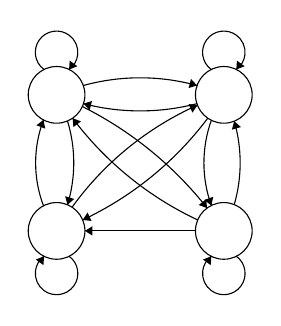
\begin{tikzpicture}[scale=0.12]
    \tikzstyle{every node}+=[inner sep=0pt]
    \draw [black] (3.2,-7.2) circle (3);
    \draw [black] (20.9,-7.2) circle (3);
    \draw [black] (3.2,-21.6) circle (3);
    \draw [black] (20.9,-21.6) circle (3);
    \draw [black] (6.03,-6.212) arc (105.44309:74.55691:22.607);
    \fill [black] (18.07,-6.21) -- (17.43,-5.52) -- (17.17,-6.48);
    \draw [black] (1.877,-4.52) arc (234:-54:2.25);
    \fill [black] (4.52,-4.52) -- (5.4,-4.17) -- (4.59,-3.58);
    \draw [black] (19.577,-4.52) arc (234:-54:2.25);
    \fill [black] (22.22,-4.52) -- (23.1,-4.17) -- (22.29,-3.58);
    \draw [black] (4.523,-24.28) arc (54:-234:2.25);
    \fill [black] (1.88,-24.28) -- (1,-24.63) -- (1.81,-25.22);
    \draw [black] (4.355,-9.963) arc (17.01386:-17.01386:15.162);
    \fill [black] (4.35,-18.84) -- (5.07,-18.22) -- (4.11,-17.93);
    \draw [black] (22.223,-24.28) arc (54:-234:2.25);
    \fill [black] (19.58,-24.28) -- (18.7,-24.63) -- (19.51,-25.22);
    \draw [black] (17.9,-21.6) -- (6.2,-21.6);
    \fill [black] (6.2,-21.6) -- (7,-22.1) -- (7,-21.1);
    \draw [black] (18.134,-20.44) arc (-115.17821:-143.08258:35.384);
    \fill [black] (4.9,-9.67) -- (4.98,-10.61) -- (5.78,-10.01);
    \draw [black] (5.932,-8.438) arc (63.42803:38.31117:39.131);
    \fill [black] (19.13,-19.18) -- (19.03,-18.24) -- (18.24,-18.86);
    \draw [black] (19.201,-9.671) arc (-36.93255:-64.80665:35.421);
    \fill [black] (5.97,-20.44) -- (6.9,-20.55) -- (6.48,-19.65);
    \draw [black] (4.842,-19.09) arc (144.19742:114.06338:32.897);
    \fill [black] (18.11,-8.3) -- (17.17,-8.17) -- (17.58,-9.08);
    \draw [black] (19.58,-18.913) arc (-160.26378:-199.73622:13.365);
    \fill [black] (19.58,-18.91) -- (19.78,-17.99) -- (18.84,-18.33);
    \draw [black] (18.051,-8.134) arc (-75.44882:-104.55118:23.886);
    \fill [black] (6.05,-8.13) -- (6.7,-8.82) -- (6.95,-7.85);
    \draw [black] (1.817,-18.946) arc (-159.19201:-200.80799:12.796);
    \fill [black] (1.82,-9.85) -- (1.07,-10.42) -- (2,-10.78);
    \draw [black] (22.003,-9.985) arc (16.17554:-16.17554:15.847);
    \fill [black] (22,-9.99) -- (21.75,-10.89) -- (22.71,-10.61);
    \end{tikzpicture}
    \end{center}
    \caption{Ergodic}
\label{fig:topologies_ergodic}
\end{figure}

\begin{figure}[!ht]
    \begin{center}
    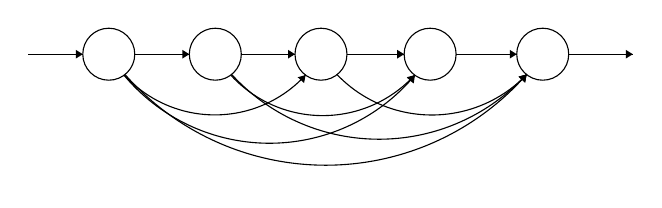
\begin{tikzpicture}[scale=0.11]
    \tikzstyle{every node}+=[inner sep=0pt]
    \draw [black] (11.5,-7.7) circle (3);
    \draw [black] (23.8,-7.7) circle (3);
    \draw [black] (36,-7.7) circle (3);
    \draw [black] (48.6,-7.7) circle (3);
    \draw [black] (61.6,-7.7) circle (3);
    \draw [black] (2.2,-7.7) -- (8.5,-7.7);
    \fill [black] (8.5,-7.7) -- (7.7,-7.2) -- (7.7,-8.2);
    \draw [black] (34.219,-10.107) arc (-42.54859:-137.45141:14.21);
    \fill [black] (34.22,-10.11) -- (33.31,-10.36) -- (34.05,-11.03);
    \draw [black] (46.84,-10.127) arc (-39.87576:-140.12424:21.878);
    \fill [black] (46.84,-10.13) -- (45.94,-10.42) -- (46.71,-11.06);
    \draw [black] (46.821,-10.108) arc (-42.43129:-137.56871:14.389);
    \fill [black] (46.82,-10.11) -- (45.91,-10.36) -- (46.65,-11.04);
    \draw [black] (59.729,-10.044) arc (-41.37756:-138.62244:30.89);
    \fill [black] (59.73,-10.04) -- (58.83,-10.31) -- (59.58,-10.97);
    \draw [black] (59.72,-10.035) arc (-42.55769:-137.44231:23.106);
    \fill [black] (59.72,-10.04) -- (58.81,-10.29) -- (59.55,-10.96);
    \draw [black] (59.748,-10.054) arc (-43.84962:-136.15038:15.181);
    \fill [black] (59.75,-10.05) -- (58.83,-10.28) -- (59.55,-10.98);
    \draw [black] (14.5,-7.7) -- (20.8,-7.7);
    \fill [black] (20.8,-7.7) -- (20,-7.2) -- (20,-8.2);
    \draw [black] (26.8,-7.7) -- (33,-7.7);
    \fill [black] (33,-7.7) -- (32.2,-7.2) -- (32.2,-8.2);
    \draw [black] (39,-7.7) -- (45.6,-7.7);
    \fill [black] (45.6,-7.7) -- (44.8,-7.2) -- (44.8,-8.2);
    \draw [black] (51.6,-7.7) -- (58.6,-7.7);
    \fill [black] (58.6,-7.7) -- (57.8,-7.2) -- (57.8,-8.2);
    \draw [black] (64.6,-7.7) -- (72,-7.7);
    \fill [black] (72,-7.7) -- (71.2,-7.2) -- (71.2,-8.2);
    \end{tikzpicture}
    \end{center}
    \caption{Left-to-right}
    \label{fig:topologies_left_to_right}
\end{figure}
\input{sections/acoustic_modeling/topologies/c}
\begin{figure}[!ht]
    \begin{center}
    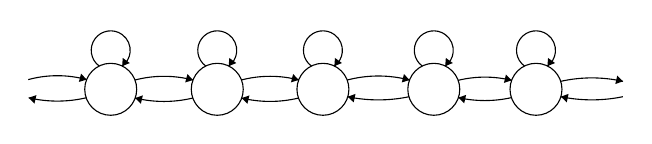
\begin{tikzpicture}[scale=0.11]
    \tikzstyle{every node}+=[inner sep=0pt]
    \draw [black] (11.5,-7.7) circle (3);
    \draw [black] (23.8,-7.7) circle (3);
    \draw [black] (36,-7.7) circle (3);
    \draw [black] (48.8,-7.7) circle (3);
    \draw [black] (60.6,-7.7) circle (3);
    \draw [black] (10.177,-5.02) arc (234:-54:2.25);
    \fill [black] (12.82,-5.02) -- (13.7,-4.67) -- (12.89,-4.08);
    \draw [black] (22.477,-5.02) arc (234:-54:2.25);
    \fill [black] (25.12,-5.02) -- (26,-4.67) -- (25.19,-4.08);
    \draw [black] (34.677,-5.02) arc (234:-54:2.25);
    \fill [black] (37.32,-5.02) -- (38.2,-4.67) -- (37.39,-4.08);
    \draw [black] (47.477,-5.02) arc (234:-54:2.25);
    \fill [black] (50.12,-5.02) -- (51,-4.67) -- (50.19,-4.08);
    \draw [black] (1.976,-6.581) arc (105.25754:74.74246:12.821);
    \fill [black] (8.72,-6.58) -- (8.08,-5.89) -- (7.82,-6.85);
    \draw [black] (14.295,-6.628) arc (104.54663:75.45337:13.357);
    \fill [black] (21,-6.63) -- (20.36,-5.94) -- (20.1,-6.91);
    \draw [black] (26.592,-6.622) arc (104.5773:75.4227:13.142);
    \fill [black] (33.21,-6.62) -- (32.56,-5.94) -- (32.31,-6.9);
    \draw [black] (38.798,-6.632) arc (104.79702:75.20298:14.105);
    \fill [black] (46,-6.63) -- (45.36,-5.94) -- (45.1,-6.91);
    \draw [black] (51.609,-6.664) arc (103.66979:76.33021:13.081);
    \fill [black] (57.79,-6.66) -- (57.13,-5.99) -- (56.9,-6.96);
    \draw [black] (63.451,-6.781) arc (102.63452:77.36548:16.452);
    \fill [black] (70.65,-6.78) -- (69.98,-6.12) -- (69.76,-7.09);
    \draw [black] (59.277,-5.02) arc (234:-54:2.25);
    \fill [black] (61.92,-5.02) -- (62.8,-4.67) -- (61.99,-4.08);
    \draw [black] (57.764,-8.662) arc (-77.38859:-102.61141:14.035);
    \fill [black] (51.64,-8.66) -- (52.31,-9.32) -- (52.53,-8.35);
    \draw [black] (45.93,-8.561) arc (-78.2626:-101.7374:17.353);
    \fill [black] (38.87,-8.56) -- (39.55,-9.21) -- (39.76,-8.23);
    \draw [black] (33.181,-8.71) arc (-76.43152:-103.56848:13.986);
    \fill [black] (26.62,-8.71) -- (27.28,-9.38) -- (27.51,-8.41);
    \draw [black] (20.98,-8.707) arc (-76.40618:-103.59382:14.169);
    \fill [black] (14.32,-8.71) -- (14.98,-9.38) -- (15.21,-8.41);
    \draw [black] (8.67,-8.679) arc (-76.81873:-103.18127:14.559);
    \fill [black] (2.03,-8.68) -- (2.7,-9.35) -- (2.92,-8.37);
    \draw [black] (70.628,-8.554) arc (-78.3068:-101.6932:17.654);
    \fill [black] (63.47,-8.55) -- (64.15,-9.21) -- (64.36,-8.23);
    \end{tikzpicture}
    \end{center}
    \caption{Bidirectional}
\label{fig:topologies_bidirectional}
\end{figure}
The second fundamental parameter of an HMM is the \textbf{prior distribution} vector, which defines the probability that a sequence of states $q_1, q_2, ..., q_T$ has of starting with each state $s_1, s_2, ..., s_K$:

$$\pi = [\pi_1, \pi_2, ..., \pi_K], \text{ where:}$$
$$\pi_i = P(q_1 = s_i), \forall i \in \{1, 2, ..., K\}.$$
The third and last parameter of HMM is the so-called \textbf{emission distribution}. As said before, an HMM has two underlying stochastic processes: an hidden and an observable one; similar to the former, the latter also produces a sequence over time, called \textit{observation sequence} $o_1, o_2, ..., o_T$.
At each time $t$, the \textbf{emission distribution} defines the probability density function (or discrete density function if the possible observation are countable) of an observation $o_t$, given the current state $s_t$:

$$e(o_t \, | \, s_t) = f_D(o_t \, | \, s_t) \text{ (continuous case) } $$

$$e(o_t \, | \, s_t) = P(o_t \, | \, s_t) \text{ (discrete case).} $$
Given a set of observations:
$$X = \{x^{(1)}, x^{(2)}, ..., x^{(m)}\}\text{, }$$
an HMM is trained with an E-M algorithm to maximize the likelihood of the observations:

$$A^*, B^*, \pi^* = \arg \max_{A, B, \pi} P(X \, | \, A, B, \pi)$$
A particularly useful application of the E-M approach to HMMs is the Viterbi algorithm, a dynamic programming algorithm originally proposed by Andrew Viterbi \cite{viterbi}, which makes possible to compute in polynomial time the most likely sequence of states, given a sequence of observations:

$$q^*_1, ..., q^*_T = \arg \max_{q_1, ..., q_T} P(q_1, ..., q_T \, | \, o_1, ..., o_T)\text{.}$$
The idea of the algorithm is to express this probability through a recurrence relationship, and then use classic dynamic programming with memoization to compute its value faster (and in polynomial time, which wouldn't be possible otherwise).
\\The recurrence relationship used to express the probability of the most likely sequence of state, given the observations $o_1, o_2, ..., o_T$ is the following:

$$V_{1, k} = P(o_1 \, | \, k) \, \pi_k, \, \forall k \in S$$
$$V_{t, k} = \max_{q \, \in \, S} P(o_t \, | \, q) \, A_{q, s_k} \, V_{t-1, q} \text{, }$$
where $A$ is the transition matrix and $\pi$ is the prior distribution. The algorithm operates as follows:

\begin{enumerate}[label=(\roman*), font=\itshape]
    \item computes the base case probabilities $V_{1, k}$ for each state $k$, storing it into a $T \times K$ matrix $V$;
    
    \item computes each remaining entry $V_{t, k}$ of the matrix according to the recurrent relationship, taking advantage of the already stored values in the matrix, and storing into another matrix $\Ptr$ the state used to compute $V_{k, t}$ (representing the most likely state to transition from, into state $s_k$ at time $t$):
    
    $$\Ptr_{t, k} = \arg \max_{q} P(o_t \, | \, q) \cdot A_{q, s_k} \cdot V_{t-1, q}$$
    
    \item computes the most likely sequence of states using the computed values in the $V$ matrix, retrieving the sequence backwards:
    
    \begin{enumerate}[label=(\alph*), font=\itshape]
        \item $q^*_T = \arg \max_q V_{T, q}$;
        \\
        \item $q^*_{t-1} = \Ptr_{t, q^*_t}$
    \end{enumerate}
\end{enumerate}



\subsection{GMM-HMM} 
Given these definitions, a GMM-HMM is a HMM where emission distribution of each state is defined by a GMM with $M$ Gaussians:

$$e(o_t \, | \, s) = P(o_t \mid \lambda)=\sum_{k=1}^{M} w_{k} \, \mathcal{N}\left(x \mid \mu_{k}, \Sigma_{k}\right),$$
Often, GMM-HMM are used to build acoustic models that represent the feature distribution of a specific class of audios, which is useful in a plenty of different tasks. In speech recognition for example, GMM-HMM acoustic models are built to represent the phoneme distribution \cite{gmmhmmspeechrecognition}, \cite{asr:dnnhmm0}, and each state corresponds to a phoneme, while in scene classification each GMM-HMM acoustic model is built to represent the audios recorded in a particular scene/context \cite{dnnhmmscene}. 

Not too differently, in SI task, which is the main subject of this study, GMM-HMM acoustic models are built to represent the audios recorded by a specific speaker. Therefore, for $p$ speakers there will be $p$ GMM-HMM models, each trained with an E-M algorithm on utterances of the corresponding speaker:

$$\HMM_1, \HMM_2, ..., \HMM_p$$
At identification time, an unknow audio $o = o_1, o_2, ..., o_T$ is scored against each GMM-HMM acoustic model using Viterbi algoritm \cite{gmmhmmspeakeridentification}, and the speaker is identified by the most likely path among all the speaker acoustic models:

$$s = \arg \max_i \Viterbi_P(o, \HMM_i) \text{, }$$
where $\Viterbi_P(o, \HMM_i)$ is the posterior probability of the most likely $\HMM_i$ state path given $o$, according to the Viterbi algorithm:

$$\Viterbi_P(o, \HMM_i) = \max_{q_1, ..., q_T} P_{i}(q_1, ..., q_T \, | \, o_1, ..., o_T)$$
This methodology has been successfully applied in multiple past studies with good results \cite{gmmhmmspeakeridentification}, alongside with the GMM-standalone acoustic modeling, which was applied to the TIMIT dataset too \cite{gmmspeakeridentification}.

As for the choice of the state number $K$ for each acoustic model, it is either chosen application domain-wise, in tasks like speech recognition where each state can represent a phoneme (e.g. triphone \cite{asr:triphone}), or can be chosen empirically through grid search methods, using instance likelihood as score.
\\The same applies to the mixture number $M$, whose optimal value can vary considerably depending on the dataset, as shown in multiple studies \cite{si:gmmhmm1}, \cite{si:gmmhmm2}, \cite{polishasr:gmmhmm}.

Finally, it is important to note that each HMM topology suits different types of tasks; in ASR, for example, letf-to-right topologies are often used, since it fits the phonetic structure of speech, which involves some phonemes before others overtime. In SI or scene classification, on the other hand, the most suitable topology turns out to be the ergodic \cite{si:dnnhmm}, \cite{dnnhmmscene}, since the structure of audio recognition patterns for these two types of task may not necessarily be ordered, as they are not related to phonemes.

\paragraph{GMM-HMM in DNN-HMM}
In DNN-HMM approach to SI, GMM-HMM acoustic models are built using feature extracted from the utterances of the training set (often MFCCs/MFCCs \& deltas \cite{si:dnnhmm}) to represent the audios recorded by each speaker, and then used with Viterbi algorithm to generate frame-level audio labels that will be later used to train the DNN model.

More specifically, for each audio $o = o_1, o_2, ..., o_T$ from the speaker $j$, where each $o_t$ is an audio frame containing some kind of feature (raw audio, power/log-scaled STFT spectrum, power/log-scaled Mel spectrum, MFCCs/ MFCCs \& deltas, LPCCs, ...), Viterbi algorithm is applied to generate the most likely state sequence (this step is sometimes also called "forced alignment" \cite{si:dnnhmm}, \cite{dnnhmmscene}):

$$q^* = q^*_1, q^*_2, ..., q^*_T = \Viterbi(o, \HMM_j) \text{, }$$
where $\Viterbi(o, \HMM_j)$ is the most likely $\HMM_j$ state path given $o$, according to the Viterbi algorithm:
$$\Viterbi(o, \HMM_j) = \arg \max_{q_1, ..., q_T} P_j(q_1, ..., q_T | o_1, ..., o_T)$$
The generated states $q^* = q^*_1, q^*_2, ..., q^*_T$ are used as frame-level labels for the audio frames $o = o_1, o_2, ..., o_T$, so that each frame $o_t$ corresponds to the state label $q^*_t$. 
\\As will be explained shortly, these labels will later be used to train the underlying DNN model used in the DNN-HMM approach.

In this study, grid search has been performed to optimize the mixture $M$ and state number $K$ of our ergodic GMM-HMM acoustic models with diagonal covariance type. Results have been varying depending on the type of features used, as shown in table \vref{tab:gmmhmmgridsearch}.

It's noteworthy that acoustic models generated using log-scaled Mel-spectrum and LPCC features were not used in later stages of the study (e.g. training of the neural network model), but were generated for comparative purposes only (although this could be subject of future studies).

\begin{footnotesize}
	\begin{table}
		\centering
		\caption{GMM-HMM grid-search Results}
		\label{tab:grid_search_results}
		\begin{tabularx}{0.5\textwidth}{Xcc}
			\toprule
			\textbf{Feature} 			& \textbf{States} & \textbf{Mixtures}    \\
			\midrule
			MFCCs \& deltas	              		& 8                      & 3         \\[0.25cm]
			LPCCs             			& 4                      & 2         \\[0.25cm]
			Log-scaled Mel Spectrum features   			& 3  					 & 2         \\ 
			\bottomrule
		\end{tabularx}
		
	\end{table}\label{tab:gmmhmmgridsearch}
	
\end{footnotesize}

	\section{DNN-HMM}\label{sec:dnnhmm}
Let's now dive into the core elements of DNN-HMM approach for SI, describing the general idea and architecture, which will be described in detail in section \vref{sec:architecture}.

The basic idea behind DNN-HMM starts from the observation that Deep Neural Networks (DNNs) are more easily capable of learning advanced, non-linear statistical relationships from input data, require a lot less preprocessing compared to GMMs, and can even work with non-independent feature frames. That being said, it seems logical and worth trying to use a DNN as an emission function of an HMM, instead of a GMM.


\subsection{Deep Neural Network (DNN)}\label{subsec:dnn}
A Deep Neural Network (DNN) is an artificial neural network that employs more than one hidden layer between the input and output layers to classify an input pattern or, more generally, learn to approximate a target function $f$. In the presence of a classification problem, such as the SI problem, an attempt is made to discriminate a pattern $x$ based on a feature $y$, which can take value among $Q$ categories (also called classes), and the DNN estimates the class probabilities $p_j, j \in \{1, ..., Q\}$. The input features to a DNN do not require special attention to preprocessing, and in fact in audio processing one can range from raw frames of audio, to MFCCs/MFCCs \& deltas, to Mel's log-scaled spectrogram features. Figure \vref{fig:dnn0} shows an example neural network for classification tasks.

\begin{figure}
	\includegraphics[width=0.5\textwidth]{images/nn}
	\caption{Deep neural network for classification with 5 output classes.}
	\label{fig:dnn0}
\end{figure}

More formally, a feed-forward DNN with $H$ layers, weight matrices $W_1, ..., W_H$, bias vectors $b_1, ..., b_H$ and activation functions $f_1, ..., f_H$ computes a non-linear function \cite{si:dnnhmm}:

$$g_{W, b}(x) := a_H(x) \text{ ,}$$
where, for $h = 1, 2, ..., H$: 

$$a_h(x) = f_h((a_{h-1}(x))^T \cdot W_h + b_h) \text{, and: }$$

$$a_0(x) = x$$
In classification tasks, the last layer activation function is often a softmax function $\sigma$, which outputs a probability $\hat{p}_j$ for each class $j$, and then the class with the highest probability is considered the predicted one:

$$q = \arg \max_j \hat{p}_j \text{, where: }$$

$$\hat{p}_j = f_H(x)_j = \sigma(x)_j := \frac{e^{x_j}}{\sum_{i=1}^{Q}e^{x_i}}$$

\paragraph{DNN training}
Generally speaking, DNN are trained to minimize a loss function $L(W, b)$ (e.g. mean squared error, mean absolute error or binary cross-entropy), and at each training cycle (so-called epochs), weights $W$ and biases $b$ are updated according to their gradient:

$$\nabla_{W, b}(L) = \Big[\frac{\partial L}{\partial b}, \frac{\partial L}{\partial W}\Big]^T \text{; }$$
while gradients are computed using the backpropagation algorithm \cite{backprogation}, the update rule for the weight based on their value can be done in many different ways, and it's in general considered a model hyperparameter to tune. Two notable and popular examples of optimization algorithms to update the network parameters are Stochastic Gradient Descent (SGD) \cite{sgd} and Adadelta \cite{adadelta}, which were also used to train the models for this work.

In multi-class classification tasks such as SI, the most used loss function is the categorical cross-entropy \cite{si:dnnhmm}:

$$L = \sum_{i=1}^{Q} p_j \log \hat{p}_j \text{, }$$
where $p_j$ is the target probability for class $j$ (usually 1 for right class, 0 otherwise) and $\hat{p}_j$ is the network-predicted probability for target class $j$.











\subsection{How DNN-HMM works}

\paragraph{DNN-HMM training}
In contrast to traditional DNN systems for IS, in those based on DNN-HMM, the network output classes do not correspond to the speakers to be identified, but to the states of each GMM-HMM acoustic model speaker generated \cite{si:dnnhmm}. As previously said, the state sequences computed from the speaker utterances with the Viterbi algorithm are used as labels for audio frames, therefore each neural network output corresponds to a GMM-HMM acoustic model state.
Hence, by minimizing the categorical cross-entropy loss function $C$ on the utterances of the training set and the corresponding labels, the network is trained to predict the posterior probabilities of each HMM state $k$, given the input audio feature frame $o_t$:

$$P(s_{t} = k \, | \, o_t)$$
In this way, the network can learn meaningful features that allow it to assign to an audio the states computed from the acoustic model of its speaker (and consequently discriminate from one speaker to another).

\paragraph{DNN-HMM decoding}
In testing stage, a new audio $o = o_1, ..., o_T$ from the test set is given as input to the neural network, which outputs a posterior probability $P(s_{t} = k \, | \, o_t)$ for each frame $o_t$. As briefly mentioned earlier, the idea behind DNN-HMM is that the neural network defines the emission probabilities of the HMM, so each posterior is converted into an emission probability (likelihood) using Bayes' theorem \cite{si:dnnhmm}:

$$e(o_t \, | \, s_{t} = k) = P(\, o_t | \, s_{t} = k) = \frac{P(s_{t} = k \, | \, o_t) P(o_t)}{P(s_{t} = k)}$$
In the previous formula, the prior probability $P(s_t = k)$ can be approximated by occurrences of state $k$ in the training utterances of the corresponding speaker, as relative frequency:

$$P(s_t = k) \approx \frac{\occurences(k)}{\statesspeakers \cdot \audiospeakers} $$
On the other hand, the (audio frame) prior probability $P(o_t)$ distribution is very hard to model without strong assumptions, but since all input frames are assumed to be independent each other, it can be considered as a constant scaling/normalization factor for the emission probability, and therefore ignored completely:

$$e(o_t \, | \, s_{t} = k) = P(\, o_t | \, s_{t} = k) = \frac{P(s_{t} = k \, | \, o_t)}{P(s_{t} = k)}$$
The last step in speaker identification task with DNN-HMM is the execution of the Viterbi decoding, where:

\begin{enumerate}[label=(\roman*), font=\itshape]
	\item $o = o_1, ..., o_T$ features against each speaker DNN-HMM model using the Viterbi algorithm, which uses the transition matrices $T_j$ and prior distributions $\pi_j$ of each speaker (from the GMM-HMM acoustic models), which gives in ouput a sequence of states $q_1, ..., q_T$ and its posterior probability:
	
	$$P_{\pi_j, T_j}(q_1, ..., q_T \, | \, o_1, ..., o_T) = \Viterbi_{P}^{\pi_j, T_j}(o)$$
	
	\item the audio is identified as belonging to the speaker DNN-HMM model which maximizes this probability:
	
	$$z^* = \arg \max_j P_{\pi_j, T_j}(q_1, ..., q_T \, | \, o_1, ..., o_T)$$
\end{enumerate}



	\section{Proposed architecture}\label{sec:architecture}
To our knowledge, the only few studies that applied DNN-HMM technique to text-independent SI tasks used deep feed-forward neural networks \cite{si:dnnhmm}, which are hardly able to capture temporal relationships between feature frames due to their sequential structure unlike, for example, Recurrent Neural Networks (RNNs).

On the other hand, as multiple studies in the SI field suggested, the use of 1D/2D Convolutional Neural Networks (CNNs) in combination with log-scaled spectrum/Mel spectrum features can greatly improve the performance of a text-independent SI system, due to the high-level feature extraction power of this type of network \cite{si:lstm}.

This simple observation led us to believe that the combination of the features extracted by both these typologies of networks could lead to even better identification performances, especially if combined to the acoustic modeling power of HMMs.

Thus, the proposed architecture is non-sequential, and combines both convolutional and recurrent layers, trying to combine both kind of features to achieve better performance.

Before describing the mentioned architecture, an overview of the most important network designs that make up its layers will be given.

\subsection{Recurrent Neural Networks (RNN)}
A recurrent neural network (RNN) is a neural network that is specialized in processing a temporal sequence of data $x_1, \cdots,x_T$.

The term "recurrent" in their name refers to the execution of the same operations on each element $x_t$ of the sequence performed by this type of network, applying the same matrix of weights $V$.

This causes each output $o_t$ to depend on the previous ones, and for the network to maintain a hidden state $h_t$ directly dependent on the previous one $h_{t-1}$.

The image \vref{fig:recurrent_neural_network_unfold} shows an RNN unfolding over time (on the sequence) in a complete network.

\begin{figure}
	\includegraphics[width=0.5\textwidth]{images/recurrent_neural_network_unfold}
	\caption{Unrolling of a basic recurrent neural network, compressed on the left and unfolded on the right, source~\cite{wiki:rnn}.}
	\label{fig:recurrent_neural_network_unfold}
\end{figure}

We are going to analyze each element of the architecture of an RNN, explaining step by step how the information is processed within this type of network:
\begin{description}
	\item[input]: $x_t$ represents the input of the network at instant $t$;
	\item[hidden state]: $h_t$ represents the hidden state at time $t$, which acts as the "memory" of the network, being computed based on $x_t$ and the previous state $h_{t-1}$ by applying weight matrices, and an activation function $f$ (any nonlinear transformation such as $\tanh$, ReLU, $\dots$) and adding a bias vector $c$:
	$$
	h_{t}=f\left(U \cdot x_{t}+V \cdot h_{t-1}+c\right)
	$$
	\item[weights]: the connections between neurons of input-to-hidden type ($x_t$ to $h_t$) are parameterized by a matrix of weights $U$, while those of hidden-to-hidden type ($h_{t-1}$ to $h_t$) and hidden-to-output type ($h_t$ to $o_t$) are respectively parameterized by two weight matrices $V$ and $W$;
	\item[output]: $o_t$ represents the output of the network, which is also often subject to a nonlinear activation function $g$, especially when the network contains other layers.
	$$
	o_{t}=g\left(b_{t}+W \cdot h_{t}\right)
	$$ 
	where $b_{t}$ is the bias vector at time $t$
\end{description}


\subsection{Long-Short-Term-Memory (LSTM)}

An LSTM is a special type of RNN. RNNs use recurrent units to learn temporal features from sequence data, as LSTMs do. However, what happens inside the recurrent unit is very different between the two, as shown in image \vref{fig:lstm}.


\begin{figure}
	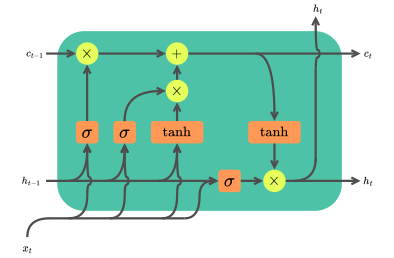
\includegraphics[width=0.5\textwidth]{images/lstm}
	\caption{LSTM unit, source \cite{wiki:lstm}.}
	\label{fig:lstm}
\end{figure}

Assuming we know the basic operation of RNNs, we are going to describe the operation of an LSTM layer at time $t$, to which comes the time sequence $x_1, x_2, \cdots, x_T$:

\begin{description}
	\item[Hidden state and input]: the hidden state of a previous time step $h_{t-1}$ and the input of the current time step $x_t$ are combined before running copies through various operational gates using concatenation between vectors.
	$$
	\left[h_{t-1} \mid x_{t}\right]
	$$
	\item[Cell state:] $c_{t-1}$ is a recurrent input representing the long-term memory of the network. In fact, it will be modified only slightly by the current time step with a sequence of linear additions and Hadamard products (component-wise), resulting in the next cell state $c_t$.
	\item[Forget gate:] this gate controls what saved information should be forgotten, and consists of a simple sigmoid neural network layer that multiplies the previous result with a weight matrix $W_f$, adds a bias vector $b_f$ and gives the result as input to a sigmoid activation function. As the sigmoid function varies between 0 and 1, it determines which cell state values should be discarded (multiplied by 0), remembered (multiplied by 1) or partially remembered (multiplied by a value between 0 and 1).
	$$
	f_{t}=\sigma\left(W_{f} \cdot\left[h_{t-1} \mid x_{t}\right]+b_{f}\right)
	$$
	\item[Input gate:] consists of a sigmoid neural layer, which multiplies [$h_{t-1} | x_t$] with a weight matrix $W_i$, adds a bias $b_i$ and gives the result as input to a sigmoid function. Outputs between 0 and 1 identify the important elements of [$h_{t-1} | x_t$] that are to be added to the cell state $c_{t-1}$.
	\item[Proposed update cell state]: consists of a $\tanh$ neural layer, which multiplies [$h_{t-1} | x_t$] with a weight a matrix $W_c$, adds a bias vector $b_c$ and gives the result as input to the activation function $\tanh$. The output $\tilde{c}_t$ determines the candidate values for storage within the cell state.
	$$
	\tilde{c}_{t}=\tanh \left(W_{c} \cdot\left[h_{t-1} \mid x_{t}\right]+b_{c}\right)
	$$
	\item[Update cell state:] the previous cell state $c_{t-1}$ is multiplied by the result of forget gate $f_t$ to remove irrelevant information, and the result is added component by component to the vector of candidate values $\tilde{c}_{t}$, weighted by the output of input gate $i_t$, to finally obtain the next cell state $c_t$.
	$$
	c_{t}=f_{t} \odot c_{t-1}+i_{t} \odot \tilde{c}_{t}
	$$
	\item[Output gate:] consists of a simple sigmoid neural layer that, again, multiplies [$h_{t-1} | x_t$] with a weight matrix $W_o$, adds a bias vector $b_o$ and gives the result in ingress to a sigmoid activation function.
	$$
	o_{t}=\sigma\left(W_{o} \cdot\left[h_{t-1} \mid x_{t}\right]+b_{o}\right)
	$$
	\item[Update hidden state:] the last step is to update the hidden-state $h_{t-1}$.  The current cell state $c_t$ is passed through the activation function $\tanh$ and multiplied component by component with the output gate result.
	$$
	o_{t}=\tanh \left(c_{t}\right) \odot o_{t}
	$$
\end{description}
Finally, the current cell state $c_t$ and hidden state $h_t$ return as input to the recurrent unit, and the process repeats until the sequence ends.

\subsection{Convolutional Neural Network (CNN)}
Convolutional neural network (CNN) is a class of artificial neural networks that has become dominant in various computer vision and signal processing tasks and is attracting interest across a variety of domains.
CNNs are capable to automatically and adaptively learn hierarchies of high-level features through layers of small weight filters representing the features.
Usually, CNN architectures are composed of multiple building blocks, such as convolution layers, batch normalization and pooling layers.


\paragraph{Convolutional Layer} 
A convolutional layer $l_m$ receives as input a signal $\boldsymbol{x}^{(m-1)}$ with $K_{m}$ channels (either raw input or the output of $(m-1)$-th layer) and computes as output a new signal $\mathbf{x}^{(m)}$ composed of $O_{m}$ channels. The output at each channel is known as a \textbf{feature map}, and is computed as \cite{cnnbook}:

$$
\boldsymbol{x}_{o}^{(m)}=g_{m}\left(\sum_{k} \boldsymbol{w}_{o,k}^{(m)}* \boldsymbol{x}_{k}^{(m-1)}+b_{o}^{(m)}\right)
$$
where $*$ denotes the 1D convolution operation:

$$
\boldsymbol{w}_{o, k} * \boldsymbol{x}_{k}[t] = \sum_{p} \boldsymbol{x}_{k}[t - p] \cdot  \boldsymbol{w}_{o, k}[p] \text{, }
$$
where $\boldsymbol{W}_{o,k}^{(m)} \in R^{P_{m}}$ is vector called \textbf{convolutional kernel}, $b_{o}^{(m)} \in \mathbb{R}$ is a bias vector and $g_m$ is the activation function applied to the final result. The convolutional kernel $\boldsymbol{w}_{o, k}^{(m)}$ act as the trainable parameters of a filter that the layer can use to detect or enhance some feature in the incoming signal frames. The weights and the consequent feature detected/enhanced by the filter are learned during the training process just like the weight matrices of fully-connected neural networks or RNN.

\paragraph{Batch Normalization Layer} 
Batch normalization is a technique that aims to accelerate the training of deep neural networks by reducing the shift of internal covariates. 
This is done through a normalization operation that fixes the means and variances of layer inputs at the batch level. This operation also has a number of extremely beneficial "side" effects:
\begin{itemize}
	\item strong reduction in the dependence of gradients on parameter scaling or their initial values, which allows much higher learning rates to be used without the risk of divergence or gradient exploding;
	\item regularization of the activation values of model units, which reduces the need for dropout or other hard-regularization techniques.
\end{itemize}
Batch normalization is applied as follows to a batch $\mathcal{B}$ with $m$ instances \cite{batchnormalization}:

\begin{enumerate}[label=(\roman*), font=\itshape]
	
	\item computes the mean and variance of the batch $\mathcal{B}$:
	
	$$
	\begin{gathered}
		\mu_{\mathcal{B}}=\frac{1}{m} \sum_{i=1}^{m} x_{i} \\
		\sigma_{\mathcal{B}}^{2}=\frac{1}{m} \sum_{i=1}^{m}\left(x_{i}-\mu_{\mathcal{B}}\right)^{2} \\
	\end{gathered}
	$$
	
	\item computes the normalized instance $\hat{x}_{i}$ for each $i \in \{1, 2, ..., m\}$:
	
	$$
	\begin{gathered}
		\hat{x}_{i} = \frac{x_{i} - \mu_{\mathcal{B}}}{\sqrt{\sigma_{\mathcal{B}}^{2} + \epsilon}} \text{, }
	\end{gathered}
	$$
	where $\epsilon$ is a very small value (e.g. machine epsilon) added to prevent division by zero.
	
	\item computes the layer output for the instance $\hat{x}_i$:
	
	$$
	\begin{gathered}
		y_{i} = \gamma \, \hat{x}_{i} + \beta = \operatorname{BN}_{\gamma, \beta}\left(x_{i}\right) \text{, }
	\end{gathered} 
	$$
	where $\gamma$ and $\beta$ are learnable parameters tuned during back-propagation.
\end{enumerate}


\paragraph{Pooling Layer}
The pooling layers of a CNN implement a dimensionality reduction transformation designed to lower the number of trainable parameters for subsequent layers, allowing them to focus on larger areas of the input patterns while retaining most of the information they contain.

Given an input signal $\boldsymbol{x}^{(m-1)}$ with $K_m$, a 1D pooling layer with pool size $P_{m} \in \mathbb{N}$ and strides $\alpha_{m} \in \mathbb{N}$ is a channel-wise operation like the following \cite{cnnbook}:

$$
\boldsymbol{x}_{o}^{(m)}[t] = \kappa \cdot \left( \sum_{p} \left(\boldsymbol{x}_{o}^{(m-1)} \left[\alpha_{m} \cdot t + p \right] \right)^{\rho}\right)^{1 / \rho}
$$
where $\kappa, \rho \in \mathbb{N}$ are fixed parameters depending on the type of pooling we are applying to the data.

It's worth noting that the use of $P_{m}=\alpha_{m}$ corresponds to dividing each channel of the input signal into non-overlapping $P_{m}$ patches (regions) and replacing the values in each region with a single value calculated on the basis of $\rho$ and $\kappa$.

In max pooling layers $(\rho = \infty, \kappa = 1)$, the output of the above formula value is the maximum of the values found in the patch:

$$
\begin{gathered}
	\lim_{\rho \to \infty} \left(\sum_{p} \left(x^{(m-1)}_o\left[\alpha_{m} \cdot t + p\right]\right)^\rho \right)^{1/\rho} = \\
	\max \left\{x^{(m-1)}_o\left[\alpha_{m} \cdot t + p\right] : p \in \{1, 2, ..., P_m\}\right\} \\
\end{gathered}
$$
In average pooling layers on the other hand, which were also used in this study, $(\rho = 1, \kappa = 1/P_m)$, the result is the average of the values:

$$
\boldsymbol{x}_{o}^{(m)}[t] = \frac{1}{P_m} \cdot \sum_{p} \boldsymbol{x}_{o}^{(m-1)} \left[\alpha_{m} \cdot t + p \right]
$$
	


\subsection{RecConvSiameseNet}\label{subsec:recconvsnet}
Let us now go into a detailed description of the neural network architecture used in the performed experiments.

\paragraph{Branches}
The proposed architecture (Figure \vref{fig:full_architecture}), named RecConvSiameseNet, involves two information processing branches:
\begin{itemize}
	\item one characterized by LSTM recurrent layers (Rec);
	\item the other featuring several 1D convolutional blocks (Conv), each containing a set of increasing 1D convolutional filters, a batch normalization layer and a 1D average pooling layer, followed by a final dense layer which flattens the feature maps extracted by the convolutional blocks.
\end{itemize}
These two branches receive as input two different types of audio features, extracted upstream during preprocessing, which are respectively:
\begin{itemize}
	\item the more refined $(243 \times 39)$ frames containing MFCCs \& deltas;
	\item the coarsest log-scaled Mel spectrum features contained in $(243 \times 128)$ frames.
\end{itemize}

The "Siamese" part in the name refers to the non-sequential nature of the network, which is typical of Siamese networks \cite{siamesenn}, although the proposed architecture does not have the usual characteristics of Siamese networks, the two branches being completely different from each other.

The basic idea, as mentioned earlier, is to combine the features that these two types of layers are capable to extract, in particular:

\begin{itemize}
	\item LSTM branch being fed with MFCCs \& deltas one $(1 \times 39)$ frame at time, and processing them in the same way, it is able to extract temporal-wise features from the cepstrum, capturing short-term and long-term relationship between frames;
	
	\item convolutional branch being fed with the $(243 \times 128)$ log-scaled Mel spectrum features in their entirety, it is capable of excerpting high-level features that span the entire audio.
\end{itemize}

\begin{figure}
	\centering
	\includegraphics[width=0.5\textwidth]{images/full_architecture}
	\caption{DNN-HMM Architecture}
	\label{fig:full_architecture}
\end{figure}
Further details on architecture and implementation of the two branches will be provided in the sections \vref{subsec:cnnautoencoder} and \vref{subsec:recautoencoder}, where the autoencoder models used during the pre-training phase will be described, as the two RecConvSiameseNet branches were extracted from them prior to the training.

\paragraph{Network tail}
As shown in the Figure \vref{fig:full_architecture}, after the feature extraction process done by the the two branches is completed, the LSTM branch result vector $u_t$ is, at each timestep $t$, concatenated with the flattened feature maps extracted by the convolutional branch $v$ (through repeat vector and concatenation layers), resulting in a new feature vector $w_t = [u_t | v]$. This feature vector is fed into a single network tail, composing of two time-distributed dense layers.

The first one has $\nspeakers \cdot \statesspeakers = 5040$ neuron units, and uses units Leaky ReLU activation function \cite{leakyrelu}, with $\alpha = 0.1$:

$$
\leakyrelu(x) := 
\begin{cases}
	x, & x \geq 0 \\
	\alpha x, & x < 0
\end{cases}
$$
The second one has $\nspeakers \cdot \statesspeakers = 5040$ neuron units too, but since it's the final output layer, it aims to predict the posterior probabilities $P(s_t = k \, | \, o_t)$ of each HMM state $k$ given the current frame $o_t$, and thus uses the softmax activation function (like the one we described in previous section \vref{subsec:dnn}).

Denoting with $W_0, b_0$ and $W_1, b_1$ the weights and biases of the first and second tail dense layers, respectively, the network output on each state can be expressed as:

$$P(s_t = k \, | \, o_t) = \sigma(a_t^T \cdot W_1 + b_1)_k \text{, where: }$$

$$a_t = \leakyrelu(w^T \cdot W_0 + b_0)$$
Details about RecConvSiameseNet training procedure and will be described in section \vref{subsec:recconvsnet_train}, while the architecture of the tail can be seen in Table \vref{tab:tail_recconvsnet}.

\begin{footnotesize}
	\begin{table}
		\centering
		\caption{Parameters of RecConvSiameseNet tail}
		\label{tab:tail_recconvsnet}
		\begin{tabularx}{0.5\textwidth}{XXr}%lMr
			\toprule
			\textbf{Layer Type} & \textbf{Parameters}                                                                   & \textbf{Shape}    \\
			\midrule
			Concatenate layer 	&  																						& (1, 243, 4.224) \\
			Dense               & 				                                                                        & (1, 243, 5040) \\[0.25cm]
			LeakyReLU			&																						& (1, 243, 5040) \\
			Dense				&   																					& (1, 243, 5040) \\
			Softmax				&																						& (1, 243, 5040) \\
			\bottomrule
		\end{tabularx}
		
	\end{table}
	
\end{footnotesize}


	
	\section{Pre-training}\label{sec:pre_training}
The concept of pre-training is inspired by human beings. Thanks to an innate ability, we don’t have to learn everything from scratch. Instead, we transfer and reuse our old knowledge of what we have learned in the past to understand new knowledge and handle a variety of new tasks.

In Deep Learning, pre-training imitates the way human beings process new knowledge. That is: using model parameters of tasks that have been learned before to initialize the model parameters of new tasks. In this way, the old knowledge helps new models successfully perform new tasks from old experience instead of from scratch.

For all these reasons, we performed pre-training on both the two branches of the previously described (\vref{sec:architecture}) neural network architecture.

\subsection{Autoencoder}

In this section, we are going to define the architecture of the CNN and LSTM autoencoders we used to pre-train the two branches of the network used in this experiment.

Autoencoders are an unsupervised artificial neural network class that learn how to efficiently encode an input vector, creating a compressed but meaningful "latent space" representation of it, in order to reconstruct it back obtaining a vector that is as close as possible to the original one. Furthermore, by design, autoencoders reduce data dimensions by learning how to ignore the noise in the data, thus they serve as very good de-noising tools.

They generally consists of four components:
\begin{description}
    \item[Encoder:] one or more stacked neural network layers $e_0, ..., e_h$ composing a function $f$, in which the model learns how to reduce the input dimensions and compress the input pattern $x$ into an encoded representation $f(x)$.
    
    \item[Bottleneck:]: the last encoder layer $e_h$, containing the compressed representation $f(x)$.
    
    \item[Decoder:] one or more stacked neural network layers $d_1, ..., d_r$ (usually, the decoder is built in a mirror-like fashion with respect to the encoder, so $r = h$, $d_1$ has the same parameters as $l_h$, $d_2$ has the same as $l_{h-1}$ and so on). These layers compose a decoder function $g$, in which the model learns how to reconstruct the original input data from the encoded representation $f(x)$ in such a way that $g(f(x))$ is as close to the original input $x$ as possible.
    
    \item[Reconstruction Loss:] exactly as in regular neural networks, autoencoders are trained with an optimization algorithm in order to minimize a loss function $J$; the only difference here is that in autoencoders the loss represents the distance between input and reconstructed output:
    $$
    J = \frac{1}{|D|} \sum_{x \in D} L(x, \hat{x}) \text{, }
    $$
    where $\hat{x}$ is the reconstruction of the network on input $x$.
    
    Often, regularization techniques such as dropout \cite{dropout} or regularization terms added to the autoencoder loss functions are used, since this has the double advantage of reducing overfitting and make the learned representation sparse, which is more suitable for different tasks other than input reconstruction, which is exactly the aim of pre-training. Another way to make the learned representation sparse is to add penalization term to the loss, based on the activation value of the bottleneck neurons:
    
    $$J = \frac{1}{|D|} \sum_{x \in D} L(x, \hat{x}) + \lambda \sum_i a^{(h)}_i \text{, }$$
    where $a^{(h)}_i$ is the activation value of the $i$-th neuron of the bottleneck.
    
    By virtue of the above, dropout and activation penalization techniques were applied to the autoencoders created for the pre-training phase of this study to make the learned audio representation as sparse as possible.
\end{description}

\subsubsection{CNN Autoencoder}\label{subsec:cnnautoencoder}
The autoencoder used to pre-train the parameters of the convolutional branch of the RecConvSiameseNet uses log-scaled Mel spectrum features extracted from each speakers'audio as input. For SI, it is important to derive features that contain the vocal characteristics of the speaker, and indeed the aim here is to provide the network with a global overview of high-level features of the audio, in contrast to the LSTM branch that aims to extract temporal-wise features.

\begin{figure}
	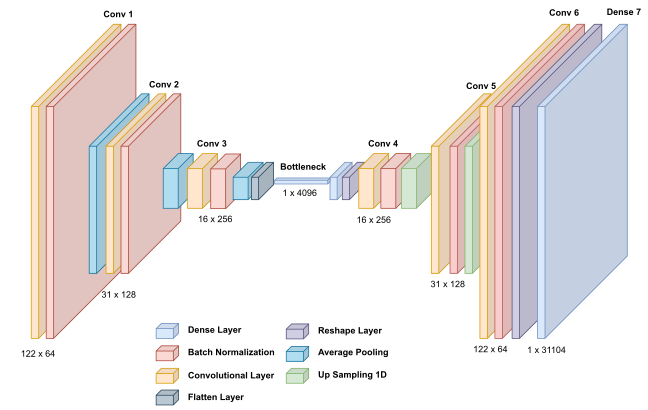
\includegraphics[width=0.5\textwidth]{images/cnn_autoencoder}
	\caption{CNN Autoencoder}
	\label{fig:cnn_autoencoder}
\end{figure}

SGD (Stochastic Gradient Descent) algorithm has been used with a learning rate of $\eta = 0.05$ to train the autoencoder for 1500 epochs with a batch size of 100 (\vref{fig:cnn_autoencoder_loss}), clipping the $L_2$ norm of the gradient to 1 and the value to of weight gradient to 0.5, in order to reduce overfitting and avoid gradient exploding.

Furthermore, as briefly mentioned before, a dropout rate of 0.5 has been applied alongside bottleneck activity regularization to prevent overfitting and make the learned data representations as sparse as possible.

\begin{figure}
	\includegraphics[width=0.5\textwidth]{images/cnn_autoencoder_graph.png}
	\caption{CNN Autoencoder Train/Validation Loss over  the first 500 epochs.}
	\label{fig:cnn_autoencoder_loss}
\end{figure}

Looking at the structure in detail, we will explore layer by layer the structure of the encoder and decoder (excluding dropout layers).

Our model's encoder consists of $3$ convolutional layers with an increasing number of filters, always followed by a batch normalization layer and by an average pooling layer that downsamples the input representation by taking the average value over the window defined by the pool size. The complete set of the encoder parameters is reported in table \vref{tab:cnn_encoder}.

\begin{footnotesize}
	\begin{table}
		\centering
		\caption{Parameters of CNN Encoder}
		\label{tab:cnn_encoder}
		\begin{tabularx}{0.5\textwidth}{XXr}%lMr
			\toprule
			\textbf{Layer Type} & \textbf{Parameters}                                                                   & \textbf{Shape} \\
			\midrule
			Input               &                                                                                       & (1, 243, 128)  \\
			Conv 1D             & \shortstack{\\ Filters, kernel, stride \\(64, 7, 2) \vphantom{space} }                & (122, 64)      \\[0.25cm]
			Batch Normalization & Features = 64                                                                         & (122, 64)      \\[0.25cm]
			Average Pooling     & Pool size = 2                                                                         & (61, 64)       \\[0.25cm] 
			Conv 1D             & \shortstack{\\ Filters, kernel, stride \\(128, 5, 2) \vphantom{space} }               & (31, 128)      \\[0.25cm]
			Batch Normalization & Features = 128                                                                        & (31, 128)      \\[0.25cm]
			Average Pooling     & Pool size = 2                                                                         & (16, 128)      \\[0.25cm]
			Conv 1D             & \shortstack{\\ Filters, kernel, stride \\(256, 5, 1) \vphantom{space} }               & (16, 256)      \\[0.25cm]
			Batch Normalization & Features = 128                                                                        & (16, 256)      \\[0.25cm]
			Average Pooling     & Pool size = 2                                                                         & (8, 256)       \\[0.25cm]
			Flatten Dense       &                                                                                       & (1, 4096)      \\
			\bottomrule
		\end{tabularx}
	\end{table}
\end{footnotesize}

The decoder is very similar to the encoder, but in reverse order, as it reconstructs the encoder’s input based on encoder’s output.

In order to match the dimension of the input, three transposed convolutional layers are needed
in the decoder in combination with upsampling layers that repeats each temporal step $r$ times along the time axis, upscaling the dimension of the reconstructed pattern, and a final triplet composed of reshape, dense and reshape layers. Decoder parameters are reported in Table \vref{tab:cnn_decoder}, while complete model architecture can be visualized in Figure \vref{fig:cnn_autoencoder}.

\begin{footnotesize}
	\begin{table}
		\centering
		\caption{Parameters of CNN Decoder}
		\label{tab:cnn_decoder}
		\begin{tabularx}{0.5\textwidth}{XXr}%lMr
			\toprule
			\textbf{Layer Type} & \textbf{Parameters}                                                                   & \textbf{Shape}    \\
			\midrule
			Dense               &                                                                         				& (1, 4096)         \\[0.25cm]
			Reshape             &                                                                                       & (16, 256)         \\[0.25cm]
			Conv 1D Transpose   & \shortstack{\\ Filters, kernel, stride \\(256, 5, 1) \vphantom{space} }               & (16, 256)         \\[0.25cm]
			Batch Normalization & Features = 256                                                                        & (16, 256)         \\[0.25cm]
			Up Sampling 1D      & Size = 2                                                                              & (32, 256)         \\[0.25cm]
			Conv 1D Transpose   & \shortstack{\\ Filters, kernel, stride \\(128, 5, 2) \vphantom{space} }               & (64, 128)         \\[0.25cm]
			Batch Normalization & Features = 128                                                                        & (64, 128)         \\[0.25cm]
			Up Sampling 1D      & Size = 2                                                                              & (128, 128)        \\[0.25cm]
			Conv 1D Transpose   & \shortstack{\\ Filters, kernel, stride \\(64, 7, 2) \vphantom{space} }                & (256, 64)         \\[0.25cm]
			Batch Normalization & Pool size = 2                                                                         & (256, 64)         \\[0.25cm]
			Reshape             &                                                                                       & (1, 16384)        \\[0.25cm]
			Dense               &                                                                          				& (1, 31104)        \\[0.25cm]
			Reshape             &                                                                                       & (1, 243, 128)     \\
			\bottomrule
		\end{tabularx}
		
	\end{table}
	
\end{footnotesize}

\subsubsection{LSTM Autoencoder}\label{subsec:recautoencoder}
The autoencoder used to pre-train the parameters of the recurrent branch of the RecConvSiameseNet takes MFCCs \& deltas features extracted from each speakers'audio as input, processing the frames one-by-one. The aim here is to extract temporal-wise features from the long-term and short-term relationships between the MFCC \& deltas frames, thanks to the memory capabilities of LSTM layers.

\begin{figure}
	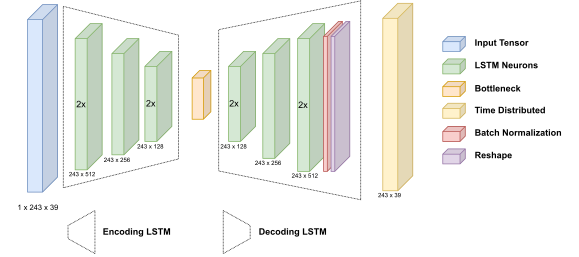
\includegraphics[width=0.5\textwidth]{images/lstm_autoencoder}
	\caption{LSTM Autoencoder}
	\label{fig:lstm_autoencoder}
\end{figure}

Adadelta algorithm has been used with a learning rate of $\eta = 1$ (as suggested by the original paper \cite{adadelta}), $\rho=0.95$ and $\epsilon=10^{-8}$ to train the LSTM autoencoder for 1000 epochs with a batch size of 200~(\vref{fig:lstm_autoencoder_loss}). 

Similar to what we have seen with the convolutional autoencoder, bottleneck activity regularization has been applied, in order to reduce overfitting and make the learned data representations as sparse as possible.

\begin{figure}
	\includegraphics[scale=0.5]{images/lstm_autoencoder_graph.png}
	\caption{LSTM Autoencoder Train/Validation Loss over the first 500 epochs.}
	\label{fig:lstm_autoencoder_loss}
\end{figure}

Diving into the architecture, encoder consists of four LSTM layers with an increasing number of units and a bottleneck of 128 units, as seen in Table~\vref{tab:lstm_encoder}.

\begin{footnotesize}
	\begin{table}
		\centering
		\caption{Parameters of LSTM Encoder}
		\label{tab:lstm_encoder}
		\begin{tabularx}{0.5\textwidth}{XXr}%lMr
			\toprule
			\textbf{Layer Type} & \textbf{Parameters}                                                                   & \textbf{Shape}    \\
			\midrule 
			LSTM               	& Units = 512	                                                                        & (243, 512)        \\[0.25cm] 
			LSTM               	& Units = 512	                                                                        & (243, 512)         \\[0.25cm] 
			LSTM               	& Units = 256	                                                                        & (243, 256)         \\[0.25cm]
			LSTM               	& Units = 128	                                                                        & (243, 128)         \\[0.25cm] 
			Bottleneck          & Dimension = 128	                                                                    &      \\ 
			\bottomrule
		\end{tabularx}
		
	\end{table}
	
\end{footnotesize}

As in the convolutional autoencoder, the decoder is built to a mirrored fashion with respect to the encoder, as we can see in the Table~\vref{tab:lstm_decoder} showing the decoder parameters. A reshape and a time distributed dense layer have been added at the end of the architecture in order to reconstruct the same shape as the fed input. The full LSTM autoencoder architecture is seen in Figure~\vref{fig:lstm_autoencoder}.

\begin{footnotesize}
	\begin{table}
		\centering
		\caption{Parameters of LSTM Decoder}
		\label{tab:lstm_decoder}
		\begin{tabularx}{0.5\textwidth}{XXr}
			\toprule
			\textbf{Layer Type} & \textbf{Parameters}                                                                   & \textbf{Shape}     \\ 
			\midrule
			LSTM               	& Units = 128	                                                                        & (243, 128)         \\[0.25cm] 
			LSTM               	& Units = 256	                                                                        & (243, 256)         \\[0.25cm] 
			LSTM               	& Units = 512	                                                                        & (243, 512)         \\[0.25cm]
			LSTM               	& Units = 512	                                                                        & (243, 512)         \\[0.25cm] 
			Batch Normalization & Features = 1024	                                                                    & (243, 1024)        \\[0.25cm]  
			Time Distributed (Dense)  	& Units = 39				                                                    & (243, 39)          \\
			\bottomrule
		\end{tabularx}
	\end{table}
\end{footnotesize}

\subsubsection{Evaluation Metrics}
Table \vref{tab:training_values_in_known_methods} illustrates the error rate analysis of the proposed autoencoders compared with some existing algorithms, such as the multiobjective evolutionary optimization algorithm~\cite{c4}, other deep convolutional and recurrent autoencoder neural networks~\cite{c5}, continual learning algorithms~\cite{c6}, enhancement parameter with a genetic algorithm~\cite{c7}, DTW~\cite{c8} and HHSAE-ASR~\cite{c9}. 

There are many possible metrics to evaluate the performances of autoencoders, but the general idea is to evaluate the reconstruction error like a distance between input and reconstructed input.

\paragraph{Mean Absolute Error}
$\mse$ evaluates the absolute distance of the observations (entries of the dataset) to the predictions on a regression, taking the average over all observations. We use the absolute value of the distances so that negative errors are accounted properly:

$$
\mae = \frac{1}{n} \sum_{i=1}^{n} \abs*{ \, \,\, y_{i}^{\text {real }}-y_{i}^{\text {pred }}}
$$

\paragraph{Mean Squared Error}
Another way to deal with negative values is by squaring the distance, so that the results are positive. This is done by the $\mse$, and higher errors (or distances) weight more in the metric than lower ones, due to the nature of the power function:

$$
\mse=\frac{1}{n} \sum_{i=1}^{n}\left(y_{i}^{\text {real }}-y_{i}^{\text {pred }}\right)^{2}
$$

\paragraph{Root Mean Squared Error}
A backlash in $\mse$ is the fact that the unit of the metric is also squared, so if the model tries to predict price in $US\$$, the $\mse$ will yield a number with unit $(US\$)^2$ which does not make sense. $\rmse$ is used then to return the $\mse$ error to the original unit by taking the square root of it, while maintaining the property of penalizing higher errors:

$$
\rmse=\sqrt{\mse}=\sqrt{\frac{1}{n} \sum_{i=1}^{n}\left(y_{i}^{\text {real }}-y_{i}^{p r e d}\right)^{2}}
$$

\paragraph{R$^2$}
It is a statistical measure in a regression model that determines the proportion of variance in the dependent variable that can be explained by the independent variable. In other words, r-squared shows how well the the regression model fits the data.
Denoting with $\bar{y}$ the mean of the real label values, and with $y_i$, $f_i$ the real label value and model prediction on $i$-th instance, respectively:
$$
\bar{y}=\frac{1}{n} \sum_{i=1}^{n} y_{i} \text{, }
$$
then the variability of the data set can be measured with two sums of squares formulas:
\begin{itemize}
	\item the sum of squares of residuals, also called the residual sum of squares:
	$$
	S S_{\text {res }}=\sum_{i}\left(y_{i}-f_{i}\right)^{2}=\sum_{i} e_{i}^{2}
	$$
	
	\item The total sum of squares (proportional to the variance of the data):
	$$
	S S_{\text {tot }}=\sum_{i}\left(y_{i}-\bar{y}\right)^{2}
	$$
\end{itemize}
That being said, the most general definition of the coefficient of determination is:

$$
R^{2}=1-\frac{S S_{\mathrm{res}}}{S S_{\mathrm{tot}}}
$$
In the best case, the modeled values exactly match the observed values, which results in $SS_{res} = 0$ and $R^2 = 1$. A baseline model, which always predicts $\bar{y}$, will have $R^2 = 0$. Models that have worse predictions than this baseline will have a negative $R^2$.

\paragraph{Analysis}
$\mse$ and $\rmse$ are very useful in understanding whether outliers generate noise in the prediction, while MAE is slightly less affected by them, so using the one or the other is a fair trade-off.\\

Optimising for $\mse$ for example, means that the generated output values are symmetrically close to the input values, meaning that an higher-than-real value is penalised by the same amount as an equally lowered one.

As for the obtained results shown in \vref{tab:training_values_in_known_methods}, it's worth noting that although the $\mae$ and $\rmse$ values of our autoencoders are particularly high if compared to the others mentioned above, this is fairly intentional and due both to the choice of not normalizing the input data, and to the applying of heavy regularization in order to make the learned weights and representations as sparse as possible and suited for usage in classification task.
Nevertheless, it's also interesting to note how both autoencoders achieve good $R^2$ values, which are satisfactorily high in the case of the convolutional one and very high in the case of the recurrent one.

\begin{footnotesize}
	\begin{table}
		\centering
		\caption{training values Error rate in Speech Processing.}
		\label{tab:training_values_in_known_methods}
		\begin{tabularx}{0.5\textwidth}{Xrrr}
			\toprule
			\textbf{Methods} 		& \shortstack{\textbf{MAE}}    	& \shortstack{\textbf{RMSE}} & \shortstack{\textbf{$R^2$}}      \\
			\midrule
			Multiobjective evolutionary\\ optimisation algorithm \cite{c4}  &N/A           & 1.43          &N/A\\
			Deep convolution\\encoder and LSTM-RNN \cite{c5}          	    &N/A           & 1.38          &N/A\\[0.25cm]
			Continual learning algorithms \cite{c6} 					    &N/A           & 1.25          &N/A\\[0.25cm]
			Genetic algorithm \cite{c7}									    &N/A           & 1.14          &N/A\\[0.25cm]
			MFCC and DTW \cite{c8}										    &N/A           & 1.12          &N/A\\[0.25cm]	
			HHSAE-ASR \cite{c9}												&N/A           & 1.087         &N/A\\[0.25cm]
			Convolutional Autoencoder\\with Mel Spectrogram				    &4.570         &6.227		   &0.8464\\[0.25cm]	
			LSTM Autoencoder\\with MFCC									    &1.796		   &2.885		   &0.9983\\
			\bottomrule
		\end{tabularx}	
	\end{table}
\end{footnotesize}

	\section{Experiment and Analysis}\label{sec:results}
Below we report the experiments performed during model training and the obtained results in the final identification phase.

\subsection{RecConvSiameseNetTraining}\label{subsec:recconvsnet_train}
Having described all previous stages, we delve now into details of the training step for the model we presented in section \vref{subsec:recconvsnet}.
RecConvSiameseNet was trained to minimize categorical cross entropy loss function for $800$ epochs with Adadelta algorithm, learning rate $\eta = 1$, $\rho=0.95$ and $\epsilon=10^{-8}$, and a batch size of $200$. Graph of training/test loss during the epochs is shown in Figure \vref{fig:recconvsnet_loss}, with the final resulting loss being $1.2096$ on the training set and $1.2071$ on the test set.

\begin{figure}
	\includegraphics[width=0.5\textwidth]{images/recconvsnet_graph.png}
	\caption{RecConvSiameseNet train/validation loss over the first 600 epochs.}
	\label{fig:recconvsnet_loss}
\end{figure}
As the network architecture is particularly complex and deep, several regularization techniques were applied to reduce overfitting and increase the generalization capabilities of the model:

\begin{itemize}
	\item for the convolutional branch: dropout rate~=~0.5;
	\item for the LSTM branch: dropout rate~=~0.7;
	\item in the first dense layer of the tail: dropout  rate~=~0.5;
	\item $L_1$ loss penalty  on the final activation values with $\lambda = 10^{-5}$;
	\item $L_1$ loss penalty on the weight values of the first dense level of the tail, with $\lambda = 10^{-5}$.
\end{itemize}

\paragraph{Evaluation metrics}
As discussed before, the network is trained using the labels generated by audio forced alignment on the GMM-HMM acoustic models with Viterbi algorithm, so it learns to estimate the posterior probabilities:

$$P(s_t = k \, | \, o_t)$$
for each state $k$, given the frame $o_t$ at each time step $t$. The training labels being artificially generated by GMM-HMM acoustic models, we surely not want the network to (hypothetically) perfectly or almost perfectly match the labels with its predictions, since this would make them completely useless, as they would be no more than an approximation of an already known model predictions (the GMM-HMM model).
It follows from this reasoning that simple accuracy cannot be used as a metric to evaluate the goodness of a neural model underlying a DNN-HMM system, since we are not interested into evaluating the exact match between network-predicted most likely state and the Viterbi-predicted ones.

What we are really interested in quantifying in this context is the model's ability to predict as most likely states those from the acoustic model of a certain speaker, given an audio $o = o_1, o_2, ..., o_T$ belonging to the latter.

The number of states of each speaker GMM-HMM acoustic model being $\statesspeakers = 8$, we used three different metrics to evaluate the performances of RecConvSiameseNet (prior to the SI step), one being widely-used and two custom ones. Each metric is calculated frame-wise, having $0$ as a minimun score and $1$ maximum score on each of them.

\begin{description}
	\item[Top-K accuracy:] the widely-used Top-K accuracy rate with $k = 8$, for each training instance frame $o_t$, it scores $1$ if the real state label $y_t$ is in the top-8 highest probability $P(s_t = q \, | \, o_t)$ values predicted by the network, and $0$ otherwise;
	
	\item[Top-K speaker accuracy:] a slightly modified Top-K accuracy rate with $k = 8$, for each training instance frame $o_t$, it scores $1$ if the real state label $y_t$ or any state label from the same speaker is in the top-8 highest probability $P(s_t = q \, | \, o_t)$ values predicted by the network, and $0$ otherwise;
	
	\item[Number of speaker states in Top-K:] a custom metric that counts, for each training instance frame $o_t$, how much states of the corresponding speaker are in the top-K most likely ones predicted by the network (with $k=8$), divided by the number of states for each speaker $\statesspeakers = 8$ (so we have 0 in case no right state is in the top-8, 0.5 if exactly 4 are, and so on).
\end{description}
Among all the above metrics, \textit{number of speaker states in top-K} is arguably the most meaningful of the three, since it carries the most information, taking into account all the states and giving all frames a different weight between 0 and 1, based on how the network performed on that specific frame. On the other hand, \textit{top-K accuracy} doesn't takes into account every state, and \textit{top-K speaker accuracy} doesn't give different weight if model predicts more than 1 speaker state in the top-K.

Table \vref{tab:reccovsnet_metrics} shows values of each presented metric for the final model, which appear to be quite high. 

\begin{footnotesize}
	\begin{table}
		\centering
		\caption{RecConvSiameseNet's metrics results}
		\begin{tabularx}{0.5\textwidth}{ccc}
			\toprule
			\textbf{Top-8} 				& \textbf{Top-8 speaker} & \textbf{\# States in top-K}    \\
			\midrule
			0.9698	              		& 0.9968                     & 0.9690         \\[0.25cm]
			\bottomrule
		\end{tabularx}
		
	\end{table}\label{tab:reccovsnet_metrics}
\end{footnotesize}

\subsection{Final results}
This brief section presents the final results of the DNN-HMM system, which appear to be comparable if not slightly better than other DNN-HMM SI systems \cite{si:dnnhmm} or LSTM/CNN-based ones \cite{si:lstm}, although the differences between the used dataset in terms of composition, dimension and distribution make comparisons very difficult. Aforementioned results are shown in Table \vref{tab:final_results}.

\begin{footnotesize}
	\begin{table}
		\centering
		\caption{Full DNN-HMM SI results}
		\begin{tabularx}{0.5\textwidth}{c}
			\toprule
			\textbf{Speaker identification accuracy}   \\
			\midrule
			0.9852	                 		\\[0.25cm]
			\bottomrule
		\end{tabularx}
	\end{table}\label{tab:final_results}
\end{footnotesize}

\subsection{Considerations and future works}
To the best of our knowledge, this is the first study that goes to apply DNN-HMM for text independent SI using a non-sequential network architecture or using both convolutional and LSTM layers.

As promising as the performances achieved are, the scope for improvement of the network and the variety of experiments that can still be carried out remains very high:

\begin{description}
	\item[Fine-tuning:] re-training the model that has already been trained on different datasets to evaluate performances of transfer learning in DNN-HMM context;
	
	\item[Parameter tweaking:] additional parameter and hyperparameter tweaking on the proposed architecture and speaker acoustic models to try improving performance even further;
	
	\item[Data augmentation:] training the model with additional augmented data to try improving the model generalization capability even more;
	
	\item[Variations of the architecture:] trying out variations of the architecture, for example replacing the current convolutional branch with more complex architectures like SincNet one \cite{si:sincnet} or other convolutional architectures;
	
	\item[Alternative/Additional features:] training the model using other typologies of features like LPCCs, or expanding the existing architectures to take advantage of them (e.g. adding a new branch);
	
	\item[Application to other datasets:] applying the same methodology and network architecture to other datasets, especially in-the-wild ones, and to the noise-added TIMIT.
\end{description}

	\section{Acknowledgements}
This research was supported by the Computer Science Department of University of Salerno, by Prof. Michele Nappi's Biometric and Image Processing Laboratory and by Ph.D. Student Chiara Pero.
	
	\printbibliography[heading=bibintoc]
	
\end{document}
